\documentclass[11pt,oneside]{article}

\usepackage[a4paper,margin=26mm,headheight=15pt]{geometry}
\usepackage[T1]{fontenc}
\usepackage[utf8]{inputenc}
\IfFileExists{libertinus.sty}{\usepackage{libertinus}}{\usepackage{lmodern}}
\usepackage{microtype}
\usepackage{amsmath,amssymb,amsthm,mathtools,mathrsfs,bm}
\usepackage{booktabs,longtable,tabularx,array}
\usepackage{graphicx}
\usepackage{xcolor}
\usepackage{enumitem}
\usepackage{fancyhdr}
\usepackage{titlesec}
\usepackage{xurl}
\usepackage{listings}
\usepackage{hyperref}
\usepackage[nameinlink,noabbrev]{cleveref}

\definecolor{linkblue}{RGB}{25,75,135}
\definecolor{deepgreen}{RGB}{24,102,72}
\definecolor{deepred}{RGB}{145,44,44}
\definecolor{shadegray}{RGB}{246,247,249}
\definecolor{rulegray}{RGB}{195,201,208}
\hypersetup{
  colorlinks=true,
  linkcolor=linkblue,
  citecolor=deepgreen,
  urlcolor=linkblue,
  pdftitle={Dyadic Primitive Ladders and Mellin--Newton Antiderivatives for the Fabius--Rvachev System},
  pdfauthor={OpenAI GPT-5.6 Pro},
  pdfsubject={Polynomial, fractional, negative, transformed, higher-order, and inverse-Fabius integral formulae},
  pdfkeywords={Fabius function, Rvachev up-function, antiderivative, Mellin transform, Newton series, inverse Fabius, Thue-Morse, q-binomial, Bell polynomial, Bernoulli polynomial, Lambert W}
}

\pagestyle{fancy}
\fancyhf{}
\fancyhead[L]{\small Dyadic primitive ladders}
\fancyhead[R]{\small\nouppercase{\leftmark}}
\fancyfoot[C]{\thepage}
\renewcommand{\headrulewidth}{0.4pt}

\titleformat{\section}{\Large\bfseries\color{linkblue}}{\thesection}{0.72em}{}
\titleformat{\subsection}{\large\bfseries\color{linkblue}}{\thesubsection}{0.65em}{}
\titleformat{\subsubsection}{\normalsize\bfseries\color{deepgreen}}{\thesubsubsection}{0.58em}{}
\setcounter{tocdepth}{2}
\setcounter{secnumdepth}{3}
\numberwithin{equation}{section}
\allowdisplaybreaks[3]
\setlength{\emergencystretch}{3em}
\setlist[itemize]{leftmargin=2em,itemsep=0.25em,topsep=0.45em}
\setlist[enumerate]{leftmargin=2.3em,itemsep=0.25em,topsep=0.45em}

\newtheorem{theorem}{Theorem}[section]
\newtheorem{proposition}[theorem]{Proposition}
\newtheorem{lemma}[theorem]{Lemma}
\newtheorem{corollary}[theorem]{Corollary}
\newtheorem{conjecture}[theorem]{Conjecture}
\newtheorem{problem}[theorem]{Open problem}
\theoremstyle{definition}
\newtheorem{definition}[theorem]{Definition}
\newtheorem{example}[theorem]{Example}
\newtheorem{algorithm}[theorem]{Algorithm}
\theoremstyle{remark}
\newtheorem{remark}[theorem]{Remark}
\newtheorem{warning}[theorem]{Warning}

\newcommand{\R}{\mathbb R}
\newcommand{\C}{\mathbb C}
\newcommand{\Q}{\mathbb Q}
\newcommand{\N}{\mathbb N}
\newcommand{\Z}{\mathbb Z}
\newcommand{\E}{\mathbb E}
\newcommand{\Prob}{\mathbb P}
\newcommand{\Up}{\operatorname{up}}
\newcommand{\sinc}{\operatorname{sinc}}
\newcommand{\wt}{s_2}
\newcommand{\dd}{\,\mathrm d}
\newcommand{\e}{\mathrm e}
\newcommand{\ii}{\mathrm i}
\newcommand{\bigO}{\mathcal O}
\newcommand{\smallo}{o}
\newcommand{\supp}{\operatorname{supp}}
\newcommand{\FP}{\operatorname{FP}}
\newcommand{\Mellin}{\mathcal M}
\newcommand{\fall}[2]{#1^{\underline{#2}}}
\newcommand{\rise}[2]{#1^{\overline{#2}}}
\newcommand{\Bell}{\mathcal B}
\newcommand{\repo}{\textsc{ProveIt}}
\newcommand{\qbinom}[3]{\genfrac{[}{]}{0pt}{}{#1}{#2}_{#3}}

\newenvironment{statusbox}[1]{%
  \par\medskip\noindent\begin{center}\begin{minipage}{0.94\textwidth}%
  \color{linkblue}\hrule\vspace{0.62em}%
  \color{black}\textbf{\color{linkblue}#1.}\ }{%
  \par\vspace{0.62em}\color{linkblue}\hrule
  \end{minipage}\end{center}\medskip}

\newenvironment{resultbox}[1]{%
  \par\medskip\noindent\begin{center}\begin{minipage}{0.94\textwidth}%
  \color{deepgreen}\hrule\vspace{0.62em}%
  \color{black}\textbf{\color{deepgreen}#1.}\ }{%
  \par\vspace{0.62em}\color{deepgreen}\hrule
  \end{minipage}\end{center}\medskip}

\newenvironment{warningbox}[1]{%
  \par\medskip\noindent\begin{center}\begin{minipage}{0.94\textwidth}%
  \color{deepred}\hrule\vspace{0.62em}%
  \color{black}\textbf{\color{deepred}#1.}\ }{%
  \par\vspace{0.62em}\color{deepred}\hrule
  \end{minipage}\end{center}\medskip}

\lstdefinestyle{python}{
  language=Python,
  basicstyle=\ttfamily\small,
  backgroundcolor=\color{shadegray},
  frame=single,
  rulecolor=\color{rulegray},
  columns=fullflexible,
  breaklines=true,
  keepspaces=true,
  showstringspaces=false,
  keywordstyle=\color{linkblue}\bfseries,
  commentstyle=\color{deepgreen},
  stringstyle=\color{deepred}
}

\title{\bfseries Dyadic Primitive Ladders and Mellin--Newton Antiderivatives\\[0.25em]
for the Fabius--Rvachev System\\[0.55em]
\large Polynomial closed forms, fractional and negative powers, transformed bumps,\\
higher-order operators, inverse quantiles, and frontier questions}
\author{Frontier research report based on the recursive \texttt{*.tex} corpus under\\
\small\path{Analysis/FabiusFunction/docs}}
\date{Pinned repository snapshot: 27 August 2026\\
\small commit \texttt{a2541a7ee373c0e297de04424f8921ce881e62b7}}

\begin{document}
\maketitle

\begin{abstract}
Let $F$ be the bounded Fabius distribution function, let $\Up$ be Rvachev's compactly
supported even bump, let $\mathcal F$ be the signed global Fabius extension, and let
$Q=F^{-1}$.  The existing \repo{} corpus develops their differential equations, exact
dyadic arithmetic, moment recurrences, half-base $q$-binomial formulae, infinite sinc
products, lower-Lambert endpoint asymptotics, and Bell--Bernoulli coefficient calculus, but
does not contain a systematic calculus for antiderivatives of monomially weighted Fabius
functions.  This report supplies such a calculus.

The key observation is an explicit primitive ladder.  If
\[
 J_m(x)=2^{\binom m2}\mathcal F(x/2^m),
\]
then $J_0=\mathcal F$ and $J_{m+1}'=J_m$.  Consequently every polynomial weight closes after
finitely many integrations by parts.  For $p\in\N$, $n\ge1$, and $0\le x\le1$ we prove
\[
 I_0^n[x^pF(x)]
 =\sum_{k=0}^{p}(-1)^k\binom pk\rise nk
 2^{\binom{n+k}{2}}x^{p-k}F(x/2^{n+k}),
\]
where $I_0^n$ is the normalized $n$-fold primitive and $\rise nk$ is a rising factorial.
The ordinary antiderivative is the case $n=1$.  A piecewise formula extends the result to
the globally bounded $F$.

For an arbitrary complex exponent $\alpha$, the finite formula becomes a normally
convergent Mellin--Newton series
\[
 I_0^n[x^\alpha F(x)]
 =\sum_{k\ge0}(-1)^k\binom\alpha k\rise nk
 2^{\binom{n+k}{2}}x^{\alpha-k}F(x/2^{n+k}).
\]
It is entire in $\alpha$, terminates exactly at nonnegative integers, and becomes a
positive-term series at negative integers.  Complete integrals are governed by the entire
moment interpolation $D(s)=\E X^s$:
\[
 \int_0^1x^\alpha F(x)\,dx
 =\frac{1-D(\alpha+1)}{\alpha+1}
 =\sum_{k\ge0}(-1)^k\binom\alpha k\frac{d_{k+1}}{k+1}.
\]
This identifies dyadic Fabius samples with forward differences in the exponent, proves
strict complete monotonicity and total positivity on the real exponent axis, and connects
the antiderivative problem directly to the sinc-product cumulants and Bell--Bernoulli
moments.

The same ladder yields shifted closed forms for $x^p\Up(x)$ on $[-1,1]$ and formulas for
the globally identical bounded-CDF transforms $x^pF(1-x)=x^p(1-F(x))$, including their
meromorphic exponent continuations.
For the inverse function we obtain the compact quantile identity
\[
 \int_0^y Q(v)^\alpha\,dv
 =yQ(y)^\alpha-\alpha\int_0^{Q(y)}x^{\alpha-1}F(x)\,dx.
\]
In particular,
\[
 \int Q(y)\,dy=yQ(y)-F\!\left(Q(y)/2\right)+C.
\]
Higher inverse primitives lead naturally to powers $F^j$, or equivalently to order
statistics of independent Fabius random variables.

Exact reciprocal-dyadic formulae, Thue--Morse and $q$-binomial substitutions, numerical
experiments, a negative-power tail model driven by the proved log-periodic endpoint
asymptotic, conjectures, a current Lean crosswalk, and a narrowed formalization plan complete
the report.  All statements are labeled as inherited, proved here, numerical, or
conjectural.  Priority outside the pinned corpus is not asserted.
\end{abstract}

\tableofcontents
\clearpage

\section{Audit boundary, novelty discipline, and claim status}
\label{sec:audit}

\subsection{Pinned corpus and reading method}

The source boundary is the exact \texttt{ProveIt} commit printed on the title page \cite{proveit}.  Its recursive documentation
tree contains 76 indexed \texttt{.tex} paths.  Every path was inventoried and searched; the
living expositions, source-paper transcriptions, archived revisions, and frontier drafts were
then grouped into mathematical lineages so that superseded copies were not mistaken for
independent results.  The families most relevant to the present problem---the primary
Fabius--Rvachev exposition, repeated-integration studies, inverse-function reports, moment and
$q$-calculus chapters, endpoint asymptotics, dyadic formulae, self-sampling/Appell material,
and spectral/frontier dossiers---were read in depth.  The full path inventory is recorded in
\cref{app:inventory}.

Targeted searches were made for \emph{antiderivative}, \emph{primitive}, \emph{monomial},
products of $F$ with powers, inverse-function areas, and candidate formula fragments such as
$F(x/2)$.  The archive does contain important repeated-integration work, but there the
iteration is applied to boxes, splines, refinements, or convolution approximants in order to
construct $\Up$; it is not a calculus of $\int x^pF(x)\,dx$.  The inverse reports concern
endpoint inversion and Lambert coordinates, not quantile antiderivatives.  The Newton-basis
frontier report concerns exponent sequences in infinite sinc products, not Newton interpolation
in the power $\alpha$ of the integrand.

\begin{warningbox}{Novelty scope}
The formula package below was not found in the pinned repository after path, phrase, and
formula searches.  This is a repository-relative novelty statement, not a claim of first
publication in the worldwide literature.  Classical ingredients such as repeated integration
by parts, Newton series, Mellin transforms, order statistics, and total positivity are of
course standard; the point is their unusually exact closure in the Fabius--Rvachev system.
\end{warningbox}

\subsection{Status convention}

The report uses four statuses.

\begin{center}
\begin{tabularx}{0.94\textwidth}{@{}>{\bfseries}lX@{}}
\toprule
Inherited & A theorem or definition already present in the pinned corpus, usually with a
matching Lean declaration.\\
Proved here & A complete paper proof is supplied below from inherited facts.  It is not
claimed to be formalized unless a later source-status note names an exact Lean declaration.\\
Numerical & A reproducible finite-precision or exact-rational experiment in the accompanying
Python program.\\
Conjectural & A statement suggested by the proved structure and experiments, with the missing
analytic step identified.\\
\bottomrule
\end{tabularx}
\end{center}

\subsection{Current Lean crosswalk for the normalized Volterra layer}

The novelty audit above remains pinned to the source snapshot on the title page.  The
following implementation-status note is later: the declarations listed here are present at
the compiled Lean checkpoint \texttt{e109088ed}, verified by a focused build.  Write
\begin{equation}
 \mathsf J_{n,a}f(x):=
 \begin{cases}
 f(x),&n=0,\\[1mm]
 \displaystyle\frac1{(n-1)!}\int_a^x(x-t)^{n-1}f(t)\,\dd t,&n>0.
 \end{cases}                                                \label{eq:lean-volterra-crosswalk}
\end{equation}
In \path{FabiusFunction.NormalizedVolterra}, the exact crosswalk is as follows.
\begin{itemize}
\item \path{normalizedVolterra_affine} is the division-free forward identity
\begin{equation}
 \mathsf J_{n,ca+d}f(cx+d)
 =c^n\mathsf J_{n,a}\bigl(t\mapsto f(ct+d)\bigr)(x).          \label{eq:lean-affine-forward}
\end{equation}
It holds for every real $c$, including $c=0$ and negative $c$, and includes $n=0$.
It has no integrability or completeness hypothesis and permits any real normed target.
\item \path{normalizedVolterra_comp_affine} is the inverse-smul form
\begin{equation}
 \mathsf J_{n,a}\bigl(t\mapsto f(ct+d)\bigr)(x)
 =(c^n)^{-1}\mathsf J_{n,ca+d}f(cx+d),\qquad c\ne0.           \label{eq:lean-affine-inverse}
\end{equation}
The nonzero-scale hypothesis is essential to this divided form.
\item \path{normalizedVolterra_basepoint_shift} states, assuming interval integrability of
$f$ from $a$ to $b$ and from $b$ to $x$,
\begin{equation}
 \mathsf J_{n,a}f(x)=\mathsf J_{n,b}f(x)
 +\sum_{k=0}^{n-1}\frac{(x-b)^k}{k!}\mathsf J_{n-k,a}f(b).    \label{eq:lean-basepoint-shift}
\end{equation}
No ordering of $a,b,x$ is imposed; at $n=0$ the sum is empty and the identity remains
valid.
\item \path{normalizedVolterra_succ_eq_taylor_of_eq_zero} states that if $f$ is interval
integrable from $a$ to $b$ and vanishes on the open unoriented interval between $b$
and $x$, then
\begin{equation}
 \mathsf J_{n+1,a}f(x)
 =\sum_{k=0}^{n}\frac{(x-b)^k}{k!}\mathsf J_{n+1-k,a}f(b).    \label{eq:lean-zero-tail}
\end{equation}
No endpoint values or endpoint ordering are required, and the vanishing hypothesis is
vacuous when $b=x$.
\end{itemize}
Thus the generic positive-order zero-tail assertion---the fact that a Volterra primitive is
a finite Taylor polynomial after the input vanishes---is formally verified.  This generic
result does not by itself identify report-specific coefficients.  Separately,
\path{normalizedVolterra_pow_mul_extendedFabius} and
\path{normalizedVolterra_pow_mul_fabiusReal_of_le_one} already formalize the signed-global
and bounded-$F$ natural-monomial coefficients (the latter on $x\le1$).  The survival,
shifted-\(\Up\), and exterior piecewise moment specializations displayed later retain the
paper-level status assigned in this report.

\subsection{Main new theorem package}

The repository search found no counterpart of the following combined package:

\begin{enumerate}
\item the dyadic primitive ladder $J_m(x)=2^{\binom m2}\mathcal F(x/2^m)$;
\item the terminating polynomial formula for every monomial and every order of integration;
\item the normally convergent complex-exponent Mellin--Newton continuation;
\item the recovery of reciprocal-dyadic samples as forward differences in the exponent;
\item complete-moment generating functions and strict total positivity of the exponent kernel;
\item shifted polynomial primitives of $\Up$ and a careful separation of $F(1-x)$ from the
      globally compact bump;
\item the inverse-quantile primitive and its higher-order order-statistic hierarchy;
\item exact dyadic formulae for weighted primitives and inverse areas;
\item the negative-power tail model obtained by combining Newton terms with the proved
      log-periodic endpoint asymptotic.
\end{enumerate}

\section{Inherited Fabius--Rvachev data and notation}
\label{sec:background}

\subsection{Three functions and one random variable}

We keep the repository's three-function convention.  Historically, the distribution goes
back to Jessen--Wintner and Fabius, while the compactly supported form was developed by the
Rvachevs \cite{jessen1935,fabius1966,rvachev1971,rvachev1990}.  The arithmetic and dyadic
normalizations used here follow the modern treatments of Arias de Reyna and Haugland
\cite{arias1982,arias2018,haugland2016}.

\begin{definition}
The \emph{bounded Fabius function} $F:\R\to[0,1]$ is zero on $(-\infty,0]$, one on
$[1,\infty)$, and on the unit interval satisfies
\begin{equation}
 F(1-x)=1-F(x),\qquad F'(x)=2F(2x)\quad(0\le x\le1/2).
 \label{eq:F-laws}
\end{equation}
The \emph{Rvachev up-function} is
\begin{equation}
 \Up(x)=F(1-|x|),\qquad \supp\Up=[-1,1].
 \label{eq:up-fold}
\end{equation}
The \emph{signed global extension} $\mathcal F$ agrees with $F$ on $[0,1]$, vanishes on the
negative half-line, and satisfies
\begin{equation}
 \mathcal F'(x)=2\mathcal F(2x)\qquad(x\in\R).
 \label{eq:global-diff}
\end{equation}
On $[-1,1]$ one has $\Up(x)=\mathcal F(x+1)$.
\end{definition}

The bounded function is the distribution function of
\begin{equation}
 X=\sum_{j=1}^{\infty}\frac{U_j}{2^j},
 \qquad U_j\stackrel{\mathrm{iid}}\sim\operatorname{Unif}[0,1].
 \label{eq:X-random}
\end{equation}
The law is symmetric: $X\stackrel d=1-X$.  Its moments are
\begin{equation}
 d_s:=D(s):=\E X^s \quad(s\in\C),\qquad d_n=D(n)\quad(n\in\N).
 \label{eq:D-def}
\end{equation}
The notation $d_s$ is used only informally for noninteger $s$; $D$ is the analytic object.
The corpus proves for integer $n\ge1$
\begin{align}
 d_n&=n\int_0^1t^{n-1}\Up(t)\,\dd t,                         \label{eq:d-survival}\\
 (n+1)(2^n-1)d_n&=\sum_{k=0}^{n-1}\binom{n+1}{k}d_k,          \label{eq:d-recurrence}\\
 F(2^{-n})&=\frac{d_n}{n!\,2^{\binom n2}}.                    \label{eq:F-reciprocal}
\end{align}
Infinite flatness at both endpoints implies that $D(s)=\E X^s$ extends to an entire function:
for every compact $K\subset\C$, the integrand $X^s$ is uniformly integrable for $s\in K$.
It also implies
\begin{equation}
 d_n=\bigO_A(n^{-A})\qquad\text{for every }A>0.                \label{eq:d-rapid}
\end{equation}
This last, deliberately weak form is enough for all Newton-series convergence arguments.

\subsection{Integral operators and factorials}

For $n\ge1$ define the normalized $n$-fold primitive from the origin by
\begin{equation}
 (I_0^nf)(x)=\frac1{(n-1)!}\int_0^x(x-t)^{n-1}f(t)\,\dd t,
 \qquad I_0^0f=f.                                             \label{eq:I0n}
\end{equation}
Thus $(I_0^nf)^{(n)}=f$, and all derivatives of orders $0,\ldots,n-1$ vanish at zero.
For a base point $a$ we similarly write
\begin{equation}
 (I_a^nf)(x)=\frac1{(n-1)!}\int_a^x(x-t)^{n-1}f(t)\,\dd t.
 \label{eq:Ian}
\end{equation}
We use
\begin{equation}
 \fall zk=z(z-1)\cdots(z-k+1),\qquad
 \rise zk=z(z+1)\cdots(z+k-1),                               \label{eq:factorials}
\end{equation}
with either product equal to $1$ at $k=0$.  Hence
$\binom zk=\fall zk/k!$ and $\rise nk=(n+k-1)!/(n-1)!$ for $n\in\N_{>0}$.

\section{The dyadic primitive ladder}
\label{sec:ladder}

\subsection{Exact closure under integration}

\begin{theorem}[Dyadic primitive ladder]
\label{thm:ladder}
For $m\in\N$ put
\begin{equation}
 J_m(x)=2^{\binom m2}\mathcal F(x/2^m).                       \label{eq:Jm}
\end{equation}
Then
\begin{equation}
 J_0=\mathcal F,\qquad J_{m+1}'=J_m,\qquad J_m^{(m)}=\mathcal F.
 \label{eq:J-ladder}
\end{equation}
For $0\le x\le1$,
\begin{equation}
 (I_0^mF)(x)=J_m(x)=2^{\binom m2}F(x/2^m).                    \label{eq:F-nprimitive}
\end{equation}
\end{theorem}

\begin{proof}
Differentiate \eqref{eq:Jm} and use \eqref{eq:global-diff}:
\[
 J_{m+1}'(x)
 =2^{\binom{m+1}{2}}2^{-(m+1)}\,2\mathcal F(x/2^m)
 =2^{\binom m2}\mathcal F(x/2^m)=J_m(x).
\]
Every $J_m$ and every derivative below order $m$ vanishes at zero because $\mathcal F$ is
flat there.  Hence $J_m$ is exactly the normalized primitive \eqref{eq:I0n}.  On the unit
interval $\mathcal F=F$ and all arguments $x/2^m$ remain in $[0,1]$.
\end{proof}

\begin{resultbox}{Interpretation}
The usual obstruction to a finite antiderivative formula is that integrating a special
function creates a new special function.  Here integration creates no new object: it only
dilates the argument by $2^{-1}$ and multiplies by a triangular power of two.  Polynomial
weights can therefore be removed by finitely many integrations by parts.
\end{resultbox}

\subsection{A useful moment bound for the ladder}

\begin{lemma}
\label{lem:J-bound}
For $m\ge1$ and $0\le x\le1$,
\begin{equation}
 0\le J_m(x)\le x^mJ_m(1)=x^m\frac{d_m}{m!}.                 \label{eq:J-bound}
\end{equation}
\end{lemma}

\begin{proof}
The Cauchy representation and monotonicity of $F$ give
\begin{align*}
 J_m(x)
 &=\frac{x^m}{(m-1)!}\int_0^1(1-u)^{m-1}F(xu)\,\dd u\\
 &\le\frac{x^m}{(m-1)!}\int_0^1(1-u)^{m-1}F(u)\,\dd u=x^mJ_m(1).
\end{align*}
If $X$ has distribution function $F$, Tonelli and symmetry yield
\[
 J_m(1)=\frac1{m!}\E(1-X)^m=\frac{d_m}{m!}.
\]
\end{proof}

This estimate is the convergence engine for the complex-exponent theory.  Notice the exact
cancellation that will later occur:
\begin{equation}
 \frac{\rise nk}{(n+k)!}=\frac1{(n-1)!(n+k)}.                 \label{eq:rising-cancel}
\end{equation}

\section{Polynomial weights: terminating closed forms}
\label{sec:polynomial}

\subsection{A polynomial theorem}

\begin{theorem}[Polynomially weighted $n$-fold primitive]
\label{thm:poly-primitive}
Let $P$ be a polynomial of degree $d$ and $n\ge1$.  On every interval on which the signed
extension is used consistently,
\begin{equation}
 \boxed{
 I_0^n[P\mathcal F](x)
 =\sum_{k=0}^{d}(-1)^k\frac{\rise nk}{k!}P^{(k)}(x)
 2^{\binom{n+k}{2}}\mathcal F(x/2^{n+k}).}
 \label{eq:poly-primitive}
\end{equation}
For $0\le x\le1$, $\mathcal F$ may be replaced by the bounded $F$ throughout.
\end{theorem}

\begin{proof}
Write $J_m=I_0^m\mathcal F$.  Repeated integration by parts gives
\[
 I_0^n[P\mathcal F]
 =\sum_{k\ge0}(-1)^k\frac{\rise nk}{k!}P^{(k)}J_{n+k}.
\]
The coefficient can be proved by induction on $k$: each new integration transfers a
derivative to $P$ and multiplies the Cauchy-kernel order by $(n+k)/(k+1)$.  Since
$P^{(k)}=0$ for $k>d$, the expansion terminates.  Substitution of \eqref{eq:Jm} proves the
formula.  One can also verify it directly by differentiating $n$ times: adjacent terms
cancel telescopically, leaving $P\mathcal F$.
\end{proof}

\subsection{Monomial formula and examples}

\begin{corollary}[Closed form for $p\in\N$]
\label{cor:monomial}
For $p\in\N$, $n\ge1$, and $0\le x\le1$,
\begin{equation}
 \boxed{
 I_0^n[x^pF(x)]
 =\sum_{k=0}^{p}(-1)^k\binom pk\rise nk
 2^{\binom{n+k}{2}}x^{p-k}F(x/2^{n+k}).}
 \label{eq:monomial-nfold}
\end{equation}
In particular, an ordinary antiderivative is
\begin{equation}
 \boxed{
 \int x^pF(x)\,\dd x
 =\sum_{k=0}^{p}(-1)^k\fall pk
 2^{\binom{k+1}{2}}x^{p-k}F(x/2^{k+1})+C.}
 \label{eq:monomial-antiderivative}
\end{equation}
\end{corollary}

The first cases are strikingly compact:
\begin{align}
 \int F(x)\,\dd x
 &=F(x/2)+C,                                                   \label{eq:example-p0}\\
 \int xF(x)\,\dd x
 &=xF(x/2)-2F(x/4)+C,                                         \label{eq:example-p1}\\
 \int x^2F(x)\,\dd x
 &=x^2F(x/2)-4xF(x/4)+16F(x/8)+C,                             \label{eq:example-p2}\\
 \int x^3F(x)\,\dd x
 &=x^3F(x/2)-6x^2F(x/4)+48xF(x/8)-384F(x/16)+C.               \label{eq:example-p3}
\end{align}
The dyadic factors $1,2,8,64,\ldots$ are $2^{\binom{k+1}{2}}$, not a geometric sequence;
the triangular exponent is forced by iterating the dilation derivative (the displayed
coefficients also contain the falling-factorial factors).

\begin{remark}[General $n$th antiderivative]
Formula \eqref{eq:monomial-nfold} is the unique $n$th antiderivative whose first $n$ Taylor
coefficients at zero vanish.  The general $n$th antiderivative is obtained by adding an
arbitrary polynomial of degree at most $n-1$.
\end{remark}

\subsection{A recurrence in the exponent}

Let
\begin{equation}
 A_\alpha(x)=\int_0^x t^\alpha F(t)\,\dd t.                   \label{eq:Aalpha}
\end{equation}
For nonnegative integer $\alpha$ this is already covered by
\eqref{eq:monomial-antiderivative}, but the recurrence below remains meaningful for every
complex exponent.

\begin{proposition}[Dilation recurrence]
\label{prop:A-recurrence}
For $0<x\le1$ and $\alpha\in\C$,
\begin{equation}
 A_\alpha(x)=x^\alpha F(x/2)-\alpha2^\alpha A_{\alpha-1}(x/2).
 \label{eq:A-recurrence}
\end{equation}
For $0<x\le1/2$ one also has
\begin{equation}
 (\alpha+1)A_\alpha(x)
 =x^{\alpha+1}F(x)-2^{-\alpha-1}A_{\alpha+1}(2x).
 \label{eq:A-functional-recurrence}
\end{equation}
\end{proposition}

\begin{proof}
For the first formula integrate by parts against the primitive $F(t/2)$ and substitute
$t=2u$ in the remaining integral.  For the second, integrate
$A_\alpha$ by parts in the opposite direction and use $F'(t)=2F(2t)$ on the left half of the
unit interval.  Infinite flatness makes the endpoint terms at zero vanish for every complex
$\alpha$.
\end{proof}

\subsection{The globally bounded \texorpdfstring{$F$}{F}: exact piecewise formula}

The signed extension is the natural object for the pure ladder, but applications often want
the bounded CDF.  The normalized primitive then has a simple piecewise completion.

\begin{theorem}[Global bounded-CDF formula]
\label{thm:global-bounded}
Let $p\in\N$ and $n\ge1$.  For $x\le0$,
\begin{equation}
 I_0^n[t^pF(t)](x)=0.                                        \label{eq:global-left}
\end{equation}
For $0\le x\le1$ use \eqref{eq:monomial-nfold}.  For $x\ge1$,
\begin{equation}
 \boxed{
 I_0^n[t^pF(t)](x)
 =\frac{p!}{(p+n)!}x^{p+n}
 -\sum_{\ell=0}^{n-1}
 \frac{(-1)^\ell x^{n-1-\ell}}{\ell!(n-1-\ell)!}
 \frac{d_{p+\ell+1}}{p+\ell+1}.}
 \label{eq:global-right}
\end{equation}
\end{theorem}

\begin{proof}
For $x\ge1$, write $F=1-(1-F)$.  The primitive of $t^p$ is the first term.  The survival
function $1-F$ is supported on $[0,1]$, so expand $(x-t)^{n-1}$ and use
\[
 \int_0^1t^m(1-F(t))\,\dd t=\frac{\E X^{m+1}}{m+1}=\frac{d_{m+1}}{m+1}.
\]
The left half-line is immediate from the bounded extension $F=0$ there.
\end{proof}

Thus outside $[0,1]$ the answer is a polynomial whose coefficients are exact rational
moments.  The apparently non-elementary content is confined to the active unit interval.

\section{Fractional, negative, and complex powers}
\label{sec:fractional}

\subsection{The Mellin--Newton expansion}

Fix the real logarithm for $x>0$, so $x^\alpha=\exp(\alpha\log x)$.

\begin{theorem}[Complex-exponent $n$-fold primitive]
\label{thm:fractional-series}
For every $n\ge1$, $0<x\le1$, and $\alpha\in\C$,
\begin{equation}
 \boxed{
 I_0^n[t^\alpha F(t)](x)
 =\sum_{k=0}^{\infty}(-1)^k\binom\alpha k\rise nk
 2^{\binom{n+k}{2}}x^{\alpha-k}F(x/2^{n+k}).}
 \label{eq:fractional-series}
\end{equation}
The series converges absolutely and locally uniformly in $\alpha$ and uniformly for $x$ in
each compact subinterval of $(0,1]$.  It therefore defines an entire function of $\alpha$.
For $\alpha=p\in\N$ it terminates and becomes \eqref{eq:monomial-nfold}.
\end{theorem}

\begin{proof}
In the Cauchy kernel \eqref{eq:I0n}, write
\[
 t^\alpha=x^\alpha\left(1-\frac{x-t}{x}\right)^\alpha
 =x^\alpha\sum_{k\ge0}(-1)^k\binom\alpha k\frac{(x-t)^k}{x^k}.
\]
On $[\epsilon,x]$ the binomial series is uniformly convergent.  Its $k$th integrated term is
\[
 (-1)^k\binom\alpha kx^{\alpha-k}\rise nk J_{n+k}(x),
\]
which is the term in \eqref{eq:fractional-series}.  To pass to zero and prove normal
convergence, apply \cref{lem:J-bound} and \eqref{eq:rising-cancel}:
\begin{align}
 \left|\binom\alpha k\rise nkx^{\alpha-k}J_{n+k}(x)\right|
 &\le
 \frac{x^{\Re\alpha+n}}{(n-1)!}
 \left|\binom\alpha k\right|\frac{d_{n+k}}{n+k}.              \label{eq:normal-bound}
\end{align}
On a compact set of exponents, $|\binom\alpha k|$ has at most polynomial growth in $k$,
whereas \eqref{eq:d-rapid} beats every polynomial.  The Weierstrass test proves all stated
forms of convergence and justifies termwise integration.
\end{proof}

For $n=1$ this reads
\begin{equation}
 \boxed{
 A_\alpha(x)=
 \sum_{k=0}^{\infty}(-1)^k\fall\alpha k
 2^{\binom{k+1}{2}}x^{\alpha-k}F(x/2^{k+1}).}
 \label{eq:A-series}
\end{equation}
The infinite series is not merely an asymptotic integration-by-parts expansion: endpoint
flatness makes it globally convergent for every complex exponent.

\subsection{Negative powers and positivity}

For $m\in\N_{>0}$, $(-1)^k\fall{-m}k=\rise mk$, so
\begin{equation}
 \boxed{
 A_{-m}(x)=\sum_{k=0}^{\infty}\rise mk
 2^{\binom{k+1}{2}}x^{-m-k}F(x/2^{k+1}).}
 \label{eq:negative-integer-series}
\end{equation}
Every term is positive.  Therefore every truncation is a rigorous lower bound, and the
remainder has no cancellation.  This is unusually favorable for certified computation.
For a general negative real exponent $\alpha=-a$, $a>0$,
\begin{equation}
 A_{-a}(x)=x^{-a}\sum_{k\ge0}\binom{a+k-1}{k}k!
 2^{\binom{k+1}{2}}x^{-k}F(x/2^{k+1}).                       \label{eq:negative-real-series}
\end{equation}
At $x=1$, the factorial and dyadic factors collapse to moments, as developed in
\cref{sec:complete}.

\begin{remark}[Why all negative powers are integrable]
Although $x^\alpha$ itself is nonintegrable at zero when $\Re\alpha\le-1$, the Fabius factor
is flatter than every power.  For each $N$ there is $C_N$ with $F(x)\le C_Nx^N$ near zero,
so $x^\alpha F(x)$ is integrable for every fixed complex $\alpha$.  The entire dependence on
$\alpha$ is a direct analytic expression of infinite flatness.
\end{remark}

\subsection{Exponent interpolation and exact forward differences}

Define
\begin{equation}
 B_{n,x}(\alpha)=x^{-\alpha}I_0^n[t^\alpha F(t)](x).           \label{eq:Bnx}
\end{equation}
Then \eqref{eq:fractional-series} is a Newton series in $\alpha$.

\begin{theorem}[Exponent--dyadic duality]
\label{thm:exponent-duality}
For $k\in\N$,
\begin{equation}
 \Delta^kB_{n,x}(0)
 =(-1)^k\rise nk2^{\binom{n+k}{2}}x^{-k}F(x/2^{n+k}),         \label{eq:forward-difference}
\end{equation}
where $\Delta h(\alpha)=h(\alpha+1)-h(\alpha)$.  Equivalently,
\begin{equation}
 \boxed{
 F(x/2^{n+k})=
 \frac{(-1)^kx^k}{\rise nk2^{\binom{n+k}{2}}}
 \Delta^kB_{n,x}(0).}
 \label{eq:recover-dyadic}
\end{equation}
At $n=x=1$,
\begin{equation}
 d_{k+1}=(-1)^k(k+1)\Delta^kM(0),\qquad
 M(\alpha):=A_\alpha(1).                                    \label{eq:mom-forward-diff}
\end{equation}
\end{theorem}

\begin{proof}
The Newton basis satisfies $\Delta^j\binom\alpha k|_{\alpha=0}=\delta_{jk}$.  Apply this to
\eqref{eq:fractional-series} after multiplication by $x^{-\alpha}$.  The last identity uses
\eqref{eq:F-reciprocal}.
\end{proof}

\begin{resultbox}{A new reconstruction principle}
Knowing the complete integral $\alpha\mapsto\int_0^1x^\alpha F(x)\,dx$ at the nonnegative
integers determines every reciprocal-dyadic sample by finite differences.  Conversely, the
reciprocal-dyadic ladder is precisely the Newton coefficient sequence of the exponent
interpolation.  Thus dyadic argument scale and discrete exponent scale are dual coordinates.
\end{resultbox}

\section{Complete integrals, moments, and special-function structure}
\label{sec:complete}

\subsection{Entire Mellin interpolation}

\begin{theorem}[Complete weighted integral]
\label{thm:complete-M}
The function
\begin{equation}
 M(\alpha)=\int_0^1x^\alpha F(x)\,\dd x                       \label{eq:M-def}
\end{equation}
is entire and satisfies
\begin{equation}
 \boxed{
 M(\alpha)=\frac{1-D(\alpha+1)}{\alpha+1}
 =\sum_{k=0}^{\infty}(-1)^k\binom\alpha k\frac{d_{k+1}}{k+1}.}
 \label{eq:M-master}
\end{equation}
The quotient has a removable singularity at $\alpha=-1$, with
\begin{equation}
 M(-1)=-D'(0)=-\E\log X=\sum_{k\ge0}\frac{d_{k+1}}{k+1}.      \label{eq:M-minus-one}
\end{equation}
For $p\in\N$,
\begin{equation}
 \int_0^1x^pF(x)\,\dd x=\frac{1-d_{p+1}}{p+1}.               \label{eq:M-integer}
\end{equation}
For $m\in\N_{>0}$,
\begin{equation}
 M(-m)=\sum_{k\ge0}\binom{m+k-1}{k}\frac{d_{k+1}}{k+1}.      \label{eq:M-negative}
\end{equation}
\end{theorem}

\begin{proof}
For $\Re\alpha>-1$, Stieltjes integration by parts gives
\[
 D(\alpha+1)=\int_0^1x^{\alpha+1}\,\dd F(x)
 =1-(\alpha+1)M(\alpha).
\]
Both sides extend entirely because of endpoint flatness, proving the first equality and the
removable value.  The second equality is \eqref{eq:fractional-series} at $n=x=1$, followed by
$2^{\binom{k+1}{2}}F(2^{-k-1})=d_{k+1}/(k+1)!$ and
$\fall\alpha k=k!\binom\alpha k$.  The integer and negative-integer cases follow.
\end{proof}

The complete $n$-fold primitive has an equally clean series.

\begin{corollary}
For $n\ge1$ and $\alpha\in\C$,
\begin{equation}
 \boxed{
 I_0^n[t^\alpha F(t)](1)
 =\frac1{(n-1)!}\sum_{k\ge0}(-1)^k\binom\alpha k
 \frac{d_{n+k}}{n+k}.}
 \label{eq:complete-nfold}
\end{equation}
\end{corollary}

\subsection{Ordinary and exponential generating functions}

Let
\begin{equation}
 G(z)=\E\e^{zX}=\sum_{n\ge0}d_n\frac{z^n}{n!}.                \label{eq:G}
\end{equation}
The corpus proves $G(2z)=((\e^z-1)/z)G(z)$.  The complete polynomial integrals have the
exponential generating function
\begin{equation}
 \boxed{
 \sum_{p\ge0}M(p)\frac{z^p}{p!}
 =\int_0^1\e^{zx}F(x)\,\dd x
 =\frac{\e^z-G(z)}{z},}
 \label{eq:M-egf}
\end{equation}
with the removable value $1/2$ at zero.  Their ordinary generating function is
\begin{equation}
 \boxed{
 \sum_{p\ge0}M(p)z^{p+1}
 =-\log(1-z)-\sum_{n\ge1}\frac{d_nz^n}{n}
 =\E\log\frac{1-zX}{1-z},\quad |z|<1.}
 \label{eq:M-ogf}
\end{equation}
For the positive half of the up-function,
\begin{equation}
 \sum_{p\ge0}z^{p+1}\int_0^1x^p\Up(x)\,\dd x
 =\E[-\log(1-zX)].                                          \label{eq:up-ogf}
\end{equation}
These identities turn moment recurrences into recurrences for whole families of weighted
antiderivatives.

\subsection{The sinc product, Bernoulli cumulants, and Bell moments}

Put $Y=2X-1$.  Its density is $\Up$ on $[-1,1]$, and its moment generating function is the
hyperbolic continuation of the infinite sinc product:
\begin{equation}
 C(z)=\E\e^{zY}
 =\prod_{j=1}^{\infty}\frac{\sinh(z/2^j)}{z/2^j}.             \label{eq:C-product}
\end{equation}
The even cumulants are
\begin{equation}
 \kappa_{2r}(Y)=\frac{2^{2r-1}B_{2r}}{r(2^{2r}-1)},
 \qquad \kappa_{2r+1}(Y)=0.                                  \label{eq:Y-cumulants}
\end{equation}
With the corpus notation
\(
 c_r=\E Y^{2r}=\int_{-1}^{1}x^{2r}\Up(x)\,\dd x,
\)
the complete exponential Bell polynomials give
\begin{equation}
 c_r=\Bell_{2r}(0,\kappa_2,0,\kappa_4,\ldots,\kappa_{2r}).    \label{eq:Bell-moments}
\end{equation}
Consequently the entire moment interpolation has the absolutely convergent Bell--Bernoulli
form
\begin{equation}
 \boxed{
 D(s)=2^{-s}\sum_{r=0}^{\infty}\binom{s}{2r}c_r
 =2^{-s}\sum_{r=0}^{\infty}\binom{s}{2r}
 \Bell_{2r}(0,\kappa_2,0,\kappa_4,\ldots,\kappa_{2r}).}
 \label{eq:D-Bell}
\end{equation}
Combining \eqref{eq:D-Bell} with \eqref{eq:M-master} expresses every fractional or negative
complete Fabius integral in Bernoulli numbers and Bell polynomials.  This is not necessarily
the fastest numerical representation, but it makes the connection with the corpus's
all-orders coefficient calculus explicit.

\subsection{Complete monotonicity and strict total positivity}

\begin{theorem}[Exponent kernel]
\label{thm:total-positive}
For real $\alpha$ and every $m\in\N$,
\begin{equation}
 (-1)^mM^{(m)}(\alpha)
 =\int_0^1x^\alpha(-\log x)^mF(x)\,\dd x>0.                  \label{eq:complete-monotone}
\end{equation}
Thus $M$ is strictly completely monotone on the whole real axis and strictly log-convex.
More strongly, if
\(a_1<\cdots<a_r\) and \(b_1<\cdots<b_r\) are real, then
\begin{equation}
 \det[M(a_i+b_j)]_{i,j=1}^r>0.                               \label{eq:strict-TP}
\end{equation}
In particular, every Hankel determinant
$\det[M(\alpha+i+j)]_{i,j=0}^{r-1}$ is positive.
\end{theorem}

\begin{proof}
Differentiation under the integral is justified by flatness, and the integrand in
\eqref{eq:complete-monotone} is positive on a set of positive measure.  Log-convexity follows
from Cauchy--Schwarz.  For total positivity, apply Andreief's identity to the positive
measure $F(x)\,\dd x$:
\begin{align*}
 \det[M(a_i+b_j)]
 =\frac1{r!}\int_{(0,1)^r}
 \det[x_j^{a_i}]\det[x_j^{b_i}]\prod_{j=1}^rF(x_j)\,\dd x_j.
\end{align*}
On the chamber $0<x_1<\cdots<x_r<1$, both generalized Vandermonde determinants have the
same strict sign; their product is positive.  The measure of that chamber is positive.
\end{proof}

\begin{remark}
The theorem supplies a large family of nonlinear inequalities among the exact values
$M(p)=(1-d_{p+1})/(p+1)$.  For example,
\[
 M(a+b)M(c+d)>M(a+d)M(c+b)
\]
whenever $a<c$ and $b<d$.  Such inequalities are invisible in the triangular moment
recurrence but automatic in the exponent-integral representation.
\end{remark}

\section{Reflection, survival, and Rvachev's up-function}
\label{sec:up}

\subsection{The two reflected bounded-CDF transforms, and the genuinely different bump}

For the bounded CDF with its constant extensions, symmetry is global:
\begin{equation}
 F(1-x)=1-F(x)\qquad(x\in\R).                                \label{eq:reflected-global}
\end{equation}
Indeed, the two sides agree by the usual symmetry on $[0,1]$, are both $1$ for $x\le0$,
and are both $0$ for $x\ge1$.  Thus the two transformations explicitly requested in the
problem have the same antiderivative theory for the bounded $F$.

The compact bump is different on the negative half-line:
\begin{equation}
 \Up(x)=F(1-|x|),\qquad
 \Up(x)=F(1-x)=1-F(x)\quad(x\ge0).                            \label{eq:three-agree}
\end{equation}
It vanishes outside $[-1,1]$, whereas the reflected/survival transform equals $1$ on
$(-\infty,0]$.  If $F$ is replaced by the signed global extension $\mathcal F$, then
$\mathcal F(1-x)$ and $1-\mathcal F(x)$ are genuinely different outside the unit interval.
Domain labels are therefore still essential.

\subsection{The survival transform \texorpdfstring{$1-F(x)$}{1-F(x)}}

\begin{theorem}[Weighted survival primitives]
\label{thm:survival}
For $p\in\N$, $n\ge1$, and $0\le x\le1$,
\begin{equation}
 I_0^n[t^pF(1-t)](x)=I_0^n[t^p(1-F(t))](x)
 =\frac{p!}{(p+n)!}x^{p+n}-I_0^n[t^pF(t)](x),                \label{eq:survival-integer}
\end{equation}
where the last term is the finite sum \eqref{eq:monomial-nfold}.  For complex $\alpha$ with
$\Re\alpha>-1$,
\begin{equation}
 I_0^n[t^\alpha F(1-t)](x)=I_0^n[t^\alpha(1-F(t))](x)
 =\frac{\Gamma(\alpha+1)}{\Gamma(\alpha+n+1)}x^{\alpha+n}
  -I_0^n[t^\alpha F(t)](x).                                  \label{eq:survival-fractional}
\end{equation}
The right side meromorphically continues to all $\alpha$, with possible simple poles at
$-1,-2,\ldots,-n$.
\end{theorem}

For $x\ge1$, the survival primitive becomes a polynomial of degree $n-1$:
\begin{equation}
 I_0^n[t^p(1-F(t))](x)
 =\sum_{\ell=0}^{n-1}
 \frac{(-1)^\ell x^{n-1-\ell}}{\ell!(n-1-\ell)!}
 \frac{d_{p+\ell+1}}{p+\ell+1}.                              \label{eq:survival-global-right}
\end{equation}
For integer $p$ and $x\le0$, since $1-F(t)=1$ along the integration path,
\begin{equation}
 I_0^n[t^p(1-F(t))](x)=\frac{p!}{(p+n)!}x^{p+n}.              \label{eq:survival-global-left}
\end{equation}

At $x=1$ the positive half of $\Up$ has the Mellin transform
\begin{equation}
 \boxed{
 U(\alpha):=\int_0^1x^\alpha\Up(x)\,\dd x
 =\frac{D(\alpha+1)}{\alpha+1}.}
 \label{eq:up-Mellin}
\end{equation}
Its meromorphic continuation has exactly one pole, at $\alpha=-1$, with residue $1$.
The finite part is
\begin{equation}
 \FP_{\alpha=-1}U(\alpha)=D'(0)
 =\int_0^1\frac{\Up(x)-1}{x}\,\dd x.                        \label{eq:up-finite-part}
\end{equation}
This one-pole simplification is a consequence of the infinite flatness of $\Up(x)-1$ at
zero.

\subsection{A shifted primitive ladder for the compact bump}

\begin{theorem}[Shifted Rvachev ladder]
\label{thm:up-ladder}
For $m\ge1$ and $-1\le x\le1$, define
\begin{equation}
 K_m(x)=2^{\binom m2}F((x+1)/2^m).                            \label{eq:Km}
\end{equation}
Then $K_1'=\Up$, $K_{m+1}'=K_m$, and $K_m$ is the normalized $m$-fold primitive from $-1$.
Consequently, for $p\in\N$ and $n\ge1$,
\begin{equation}
 \boxed{
 I_{-1}^n[t^p\Up(t)](x)
 =\sum_{k=0}^{p}(-1)^k\binom pk\rise nk
 2^{\binom{n+k}{2}}x^{p-k}F((x+1)/2^{n+k}).}
 \label{eq:up-monomial}
\end{equation}
\end{theorem}

\begin{proof}
On the support, $\Up(x)=\mathcal F(x+1)$.  Shift the global ladder of
\cref{thm:ladder}; for $m\ge1$ the argument $(x+1)/2^m$ lies in $[0,1]$, so the bounded $F$
is sufficient.  The polynomial formula follows exactly as in \cref{thm:poly-primitive}, now
with base point $-1$.
\end{proof}

For fractional powers on the negative half of the support, it is natural to use $(-x)^\alpha$.
If $-1<x<0$, substitution $u=x+1$ and a uniformly convergent binomial series give
\begin{equation}
 \boxed{
 \int_{-1}^{x}(-t)^\alpha\Up(t)\,\dd t
 =\sum_{k=0}^{\infty}(-1)^k\binom\alpha k A_k(1+x).}
 \label{eq:up-negative-half-fractional}
\end{equation}
At $x=0$ the formula continues for $\Re\alpha>-1$ and then meromorphically.  The even Mellin
transform of the full bump is
\begin{equation}
 \int_{-1}^1|x|^\alpha\Up(x)\,\dd x
 =\frac{2D(\alpha+1)}{\alpha+1}.                             \label{eq:up-even-Mellin}
\end{equation}

\section{Higher derivatives and mixed orders}
\label{sec:derivatives}

\subsection{Derivatives of monomially weighted Fabius functions}

The corpus gives
\begin{equation}
 F^{(j)}(x)=2^{\binom{j+1}{2}}\mathcal F(2^jx)\qquad(0<x<1).
 \label{eq:F-derivative-ladder}
\end{equation}
Leibniz's rule immediately gives the derivative companion to the primitive formula.

\begin{theorem}[Closed derivative formula]
\label{thm:weighted-derivative}
For $n\in\N$, $\alpha\in\C$, and $0<x<1$,
\begin{equation}
 \boxed{
 \frac{\dd^n}{\dd x^n}\bigl(x^\alpha F(x)\bigr)
 =\sum_{j=0}^{n}\binom nj\fall\alpha{n-j}
 x^{\alpha-n+j}2^{\binom{j+1}{2}}\mathcal F(2^jx).}
 \label{eq:weighted-derivative}
\end{equation}
On $-1<x<1$, replace the final factor by
$\mathcal F(2^j(x+1))$ to obtain the corresponding formula for $x^\alpha\Up(x)$ on a chosen
branch of $x^\alpha$.
\end{theorem}

Thus positive and negative operator orders are both finite on polynomial weights: positive
orders use expanding dyadic arguments, while antiderivatives use contracting arguments.  The
signed extension is the common carrier that makes both directions globally meaningful.

\subsection{A bilateral operator notation}

For integer $r$ define $\mathscr D^r$ by ordinary differentiation when $r\ge0$ and by the
normalized primitive $I_0^{-r}$ when $r<0$.  For a monomial weight $x^p$, both signs of $r$
produce finite sums.  A useful research question is whether there is a natural fractional
operator $\mathscr D^z$ satisfying a dyadic semigroup law and interpolating both
\eqref{eq:fractional-series} and \eqref{eq:weighted-derivative}.  Classical
Riemann--Liouville operators interpolate in the order of integration, whereas the present
Newton series interpolates in the exponent of the monomial.  The two complex parameters
should be studied jointly.

\section{Integrals and derivatives of the inverse Fabius function}
\label{sec:inverse}

\subsection{The quantile area identity}

Let $Q=F^{-1}:[0,1]\to[0,1]$.  Strict monotonicity on the open unit interval and endpoint
continuity are inherited from the corpus.

\begin{theorem}[Inverse-power primitive]
\label{thm:inverse-master}
For $0<y\le1$, put $q=Q(y)$.  Then for every $\alpha\in\C$,
\begin{equation}
 \boxed{
 \mathcal Q_\alpha(y):=\int_0^yQ(v)^\alpha\,\dd v
 =yq^\alpha-\alpha A_{\alpha-1}(q).}
 \label{eq:inverse-master}
\end{equation}
Both sides are entire in $\alpha$.  At $y=0$ the common continuous value is $0$; this endpoint is understood by continuation rather than by the indeterminate symbol $0^\alpha$.  At $y=1$,
\begin{equation}
 \int_0^1Q(v)^\alpha\,\dd v=D(\alpha).                       \label{eq:inverse-complete}
\end{equation}
\end{theorem}

\begin{proof}
Substitute $v=F(x)$ in the Lebesgue--Stieltjes sense:
\[
 \int_0^yQ(v)^\alpha\,\dd v=\int_0^qx^\alpha\,\dd F(x).
\]
Integration by parts gives $q^\alpha F(q)-\alpha\int_0^qx^{\alpha-1}F(x)\,\dd x$.
The endpoint term at zero vanishes for every complex exponent because $F$ is infinitely
flat.  Since $F(q)=y$, this is \eqref{eq:inverse-master}.  The complete identity is the
quantile representation of moments.
\end{proof}

\begin{corollary}[An elementary-looking inverse antiderivative]
\label{cor:inverse-one}
An ordinary antiderivative of $Q$ is
\begin{equation}
 \boxed{
 \int Q(y)\,\dd y
 =yQ(y)-F\!\left(\frac{Q(y)}2\right)+C.}
 \label{eq:inverse-one}
\end{equation}
More generally, for $p\in\N_{>0}$,
\begin{align}
 \int_0^yQ(v)^p\,\dd v
 ={}&yq^p
 -p\sum_{k=0}^{p-1}(-1)^k\fall{p-1}k
 2^{\binom{k+1}{2}}q^{p-1-k}F(q/2^{k+1}).                   \label{eq:inverse-integer}
\end{align}
Differentiating \eqref{eq:inverse-master} at $\alpha=0$ gives
\begin{equation}
 \int_0^y\log Q(v)\,\dd v=y\log q-A_{-1}(q).                \label{eq:inverse-log}
\end{equation}
\end{corollary}

Formula \eqref{eq:inverse-one} is the exact area-under-an-inverse identity specialized to the
Fabius primitive ladder.  Its compactness is a useful diagnostic: differentiating the right
side, the two $Q'$ terms cancel because
$\tfrac12F'(Q/2)=F(Q)=y$.

For negative complete inverse powers,
\begin{equation}
 D(-m)=1+mM(-m-1)
 =1+m\sum_{k\ge0}\binom{m+k}{k}\frac{d_{k+1}}{k+1}.           \label{eq:inverse-negative-complete}
\end{equation}
Again the series has positive terms.

\subsection{Weighted inverse integrals and the nonlinear hierarchy}

\begin{proposition}[Beta-weighted quantiles]
\label{prop:weighted-inverse}
For $r\in\N$, $0<y\le1$, $q=Q(y)$, and $\alpha\in\C$,
\begin{equation}
 \boxed{
 \int_0^yv^rQ(v)^\alpha\,\dd v
 =\frac{y^{r+1}q^\alpha}{r+1}
 -\frac{\alpha}{r+1}\int_0^qx^{\alpha-1}F(x)^{r+1}\,\dd x.}
 \label{eq:weighted-inverse}
\end{equation}
\end{proposition}

\begin{proof}
After $v=F(x)$, write $F(x)^r\,\dd F(x)=\dd(F(x)^{r+1})/(r+1)$ and integrate by parts.
\end{proof}

This introduces
\begin{equation}
 H_{\beta,j}(q)=\int_0^qx^\beta F(x)^j\,\dd x,                \label{eq:H-hierarchy}
\end{equation}
a nonlinear hierarchy absent from the linear primitive ladder.  Expanding the Cauchy kernel
and using \eqref{eq:weighted-inverse} yields:

\begin{theorem}[Higher inverse primitive]
\label{thm:inverse-nfold}
For $n\ge1$,
\begin{equation}
 \boxed{
 I_0^n[Q^\alpha](y)
 =\frac{y^nq^\alpha}{n!}
 -\frac{\alpha}{n!}\sum_{j=1}^{n}(-1)^{j-1}\binom nj
 y^{n-j}H_{\alpha-1,j}(q).}
 \label{eq:inverse-nfold}
\end{equation}
\end{theorem}

The linear Fabius ladder therefore solves the first inverse primitive completely, but higher
inverse primitives expose powers of $F$.  This is not a failure of the method: it identifies
the exact new objects required at the next level.

\subsection{Order-statistic interpretation}

Let $X_1,\ldots,X_n$ be independent copies of $X$.

\begin{theorem}[Order statistics]
\label{thm:order-statistics}
For real parts in the domain of the displayed expectation,
\begin{equation}
 I_0^n[Q^\alpha](1)
 =\frac1{n!}\E\left[\min(X_1,\ldots,X_n)^\alpha\right].       \label{eq:min-order}
\end{equation}
For $\Re\alpha>0$ this is
\begin{equation}
 I_0^n[Q^\alpha](1)
 =\frac{\alpha}{n!}\int_0^1t^{\alpha-1}(1-F(t))^n\,\dd t
 =\frac{\alpha}{n!}\int_0^1t^{\alpha-1}\Up(t)^n\,\dd t.    \label{eq:min-survival}
\end{equation}
In particular,
\begin{equation}
 I_0^nQ(1)=\frac1{n!}\int_0^1\Up(t)^n\,\dd t.                \label{eq:inverse-up-power}
\end{equation}
More generally, for $r,s\in\N$,
\begin{equation}
 \int_0^1y^r(1-y)^sQ(y)^\alpha\,\dd y
 =B(r+1,s+1)\,
 \E\left[X_{(r+1:r+s+1)}^\alpha\right].                     \label{eq:beta-order}
\end{equation}
\end{theorem}

\begin{proof}
The minimum of $n$ independent uniform variables has density
$n(1-y)^{n-1}$; applying the quantile map $Q$ gives the minimum of $n$ independent Fabius
variables.  The survival formula for a positive power gives \eqref{eq:min-survival}.  The
Beta density yields \eqref{eq:beta-order}.
\end{proof}

This probabilistic interpretation suggests studying the nonlinear integrals of $F^j$ through
order statistics rather than through direct functional equations.

\subsection{Derivatives of the inverse}

For $0<y<1$ and $q=Q(y)$,
\begin{equation}
 Q^{(n)}(y)=
 \left[\left(\frac1{F'(x)}\frac{\dd}{\dd x}\right)^{n-1}
 \frac1{F'(x)}\right]_{x=q}.                                 \label{eq:inverse-derivatives}
\end{equation}
Fa\`a di Bruno's formula then gives
\begin{equation}
 \frac{\dd^n}{\dd y^n}Q(y)^\alpha
 =\sum_{k=1}^n\fall\alpha kQ(y)^{\alpha-k}
 B_{n,k}\bigl(Q',Q'',\ldots,Q^{(n-k+1)}\bigr),               \label{eq:inverse-power-derivative}
\end{equation}
where $B_{n,k}$ are partial Bell polynomials.  Combining
\eqref{eq:inverse-derivatives} with the Fabius derivative ladder expresses every derivative
in terms of $q$, $\mathcal F(2^jq)$, and rational operations.  Endpoint blow-up is encoded by
the reciprocal factors $1/F'(q)$ and is naturally analyzed in the lower-Lambert coordinate
already developed in the corpus.

\section{Exact dyadic arithmetic, Thue--Morse sums, and \texorpdfstring{$q$}{q}-binomials}
\label{sec:dyadic}

\subsection{Reciprocal-dyadic weighted primitives}

\begin{theorem}[Exact reciprocal-dyadic formula]
\label{thm:dyadic-primitive}
For $p,r\in\N$ and $n\ge1$,
\begin{equation}
 \boxed{
 I_0^n[x^pF(x)](2^{-r})
 =2^{-r(n+p)-\binom r2}
 \sum_{k=0}^{p}(-1)^k\binom pk\rise nk
 \frac{d_{r+n+k}}{(r+n+k)!}.}
 \label{eq:dyadic-primitive}
\end{equation}
In particular the value is rational.
\end{theorem}

\begin{proof}
Insert $x=2^{-r}$ into \eqref{eq:monomial-nfold}, then use
\eqref{eq:F-reciprocal} at index $r+n+k$.  The power of two in each summand is
\[
 2^{-r(p-k)}2^{\binom{n+k}{2}-\binom{r+n+k}{2}}
 =2^{-r(n+p)-\binom r2},
\]
independent of $k$.  This cancellation is the arithmetic signature of the primitive ladder.
\end{proof}

\subsection{Exact inverse areas at reciprocal-dyadic ordinates}

If $q=2^{-r}$ and $y=F(q)$, then \eqref{eq:inverse-integer} simplifies similarly.

\begin{theorem}[Dyadic quantile area]
\label{thm:dyadic-inverse-area}
For $p\in\N_{>0}$ and $r\in\N$,
\begin{equation}
 \boxed{
 \int_0^{F(2^{-r})}Q(v)^p\,\dd v
 =2^{-rp-\binom r2}
 \left[
 \frac{d_r}{r!}
 -p\sum_{k=0}^{p-1}(-1)^k\fall{p-1}k
 \frac{d_{r+k+1}}{(r+k+1)!}
 \right].}
 \label{eq:dyadic-inverse-area}
\end{equation}
\end{theorem}

At $r=2$, $q=1/4$, $y=F(q)=5/72$, the first six exact values are
\begin{center}
\begin{tabular}{@{}cl@{}}
\toprule
$p$ & $\displaystyle\int_0^{5/72}Q(v)^p\,\dd v$\\
\midrule
1 & $1/72$\\
2 & $1493/518400$\\
3 & $53/86400$\\
4 & $48781/365783040$\\
5 & $10777/365783040$\\
6 & $196806103/29847896064000$\\
\bottomrule
\end{tabular}
\end{center}
These were evaluated independently by exact rational arithmetic and checked by numerical
quantile quadrature.

\subsection{Arbitrary dyadic arguments and Thue--Morse signs}

The corpus proves, for $0\le a\le2^N$,
\begin{equation}
 F(a/2^N)=\frac{2^{-\binom{N+1}{2}}}{N!}
 \sum_{h=0}^{a-1}(-1)^{\wt(h)}
 \sum_{j=0}^{\lfloor N/2\rfloor}\binom N{2j}c_j
 (2a-2h-1)^{N-2j}.                                          \label{eq:repo-dyadic}
\end{equation}
Putting $x=a/2^r$ in \eqref{eq:monomial-nfold} and applying
\eqref{eq:repo-dyadic} with $N=r+n+k$ gives an entirely finite closed form for every
weighted primitive at every dyadic argument.  It involves only rational centered moments
$c_j$, binomial coefficients, powers of two, and the signed Thue--Morse sequence
$(-1)^{\wt(h)}$.  We leave it in this compositional form because expanding the three finite
sums obscures the ladder structure and offers no computational advantage.

Write
\begin{equation}
 (a;q)_N=\prod_{\ell=0}^{N-1}(1-aq^\ell),\qquad
 \qbinom Njq=\frac{(q;q)_N}{(q;q)_j(q;q)_{N-j}},              \label{eq:q-notation}
\end{equation}
with the usual empty-product convention \cite{gasper2004}.  The alternative translated
half-base $q$-binomial identity in the corpus is, for $m,N\in\N$,
\begin{align}
 \mathcal F(m/2^N)
 &=\frac{1}{2^{N^2}(1/2;1/2)_N}
 \sum_{j=0}^{N}
 \frac{\qbinom Nj{1/2}}{4^{\binom j2}(N+j)!}
 \sum_{h=0}^{m2^j-1}(-1)^{\wt(h)}(h-m2^j+R)^{N+j},            \label{eq:repo-q-dyadic}
\end{align}
independent of the translation parameter $R\in\C$.  Substitution of
\eqref{eq:repo-q-dyadic} into each ladder term supplies a $q$-binomial version of the
antiderivative formula.  This explains how $q$-Pochhammer symbols enter the integral problem:
not through integration itself, which is elementary in the ladder basis, but through exact
evaluation of the contracted Fabius samples.

\section{Numerical experiments and reproducibility}
\label{sec:numerics}

\subsection{Independent representations}

The accompanying program \path{fabius_integrals_experiments.py} uses two independent
representations.

\begin{enumerate}
\item A dyadic grid with $2^{18}+1=262145$ nodes is iterated under the integral/reflection
      fixed point for $F$.  This checks pointwise finite primitives, shifted up-primitives,
      and inverse-quantile areas.
\item The exact rational recurrence \eqref{eq:d-recurrence} and a separate floating version
      through $d_{900}$ check complete Newton sums, exact dyadic values, and negative-power
      tails without differentiating a flat function numerically.
\end{enumerate}

The principal error maxima in the default run were
\begin{center}
\begin{tabular}{@{}lr@{}}
\toprule
Test family & maximum absolute discrepancy\\
\midrule
Finite $F$ primitive versus direct quadrature & $1.85\times10^{-10}$\\
Shifted $\Up$ primitive versus direct quadrature & $2.39\times10^{-7}$\\
Exact dyadic inverse areas versus quantile quadrature & $4.04\times10^{-9}$\\
Grid value $F(1/4)$ versus $5/72$ & $3.23\times10^{-12}$\\
\bottomrule
\end{tabular}
\end{center}
The larger up-error is caused by direct quadrature across a compact-support endpoint and by
interpolation, not by instability of the closed form.

\subsection{Fractional and negative complete integrals}

With 900 moment terms the computed values include
\begin{center}
\begin{tabular}{@{}lr@{}}
\toprule
$\alpha$ & $M(\alpha)=\int_0^1x^\alpha F(x)\,\dd x$\\
\midrule
$-2$ & $1.3148861440026451$\\
$-1$ & $0.7582400004044057$\\
$-1/2$ & $0.6073863107431697$\\
$1/2$ & $0.4209681733402678$\\
$3/2$ & $0.3146395582080128$\\
$\sqrt2$ & $0.3218439940718418$\\
\bottomrule
\end{tabular}
\end{center}
Grid quadrature agrees to roughly $10^{-9}$ or better in these tests despite the negative
powers.

\IfFileExists{newton_series_convergence.png}{%
\begin{figure}[htbp]
\centering
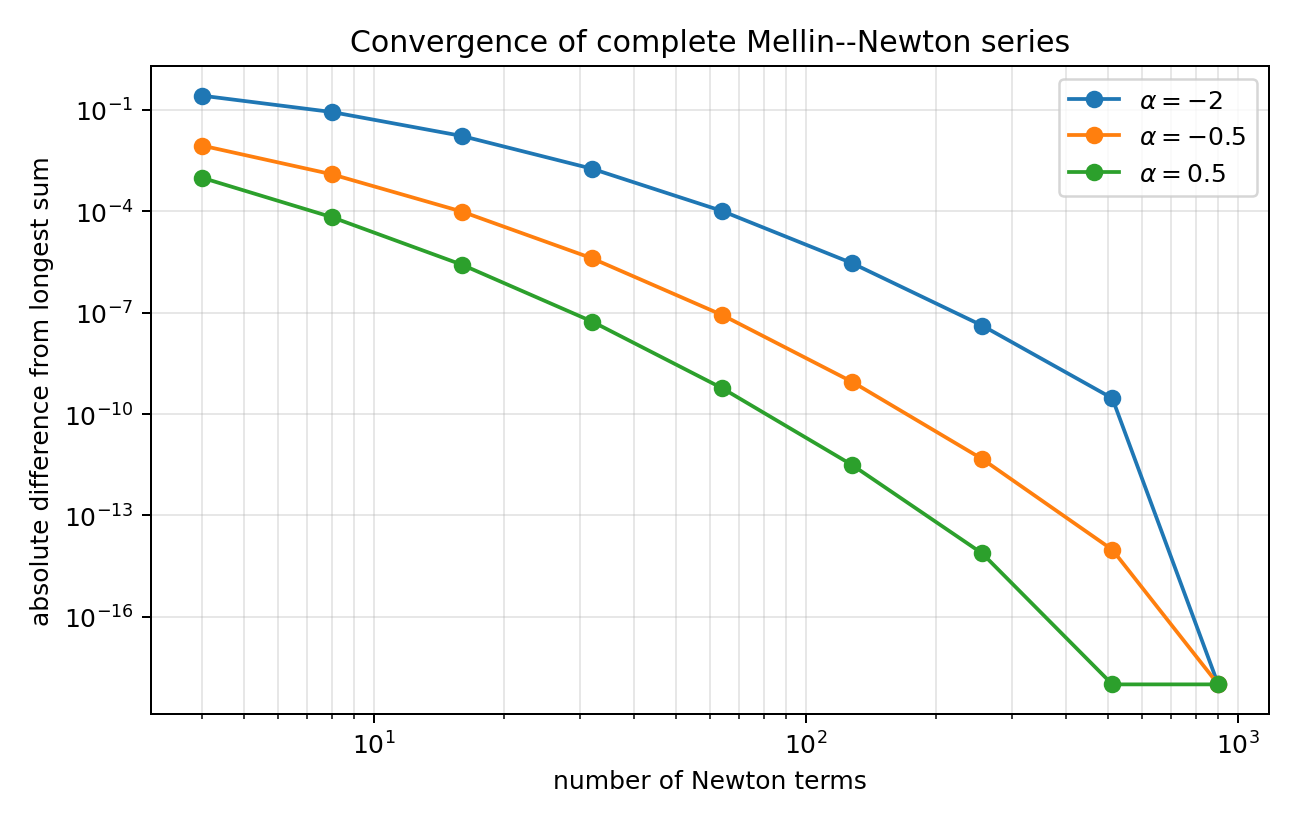
\includegraphics[width=0.82\textwidth]{newton_series_convergence.png}
\caption{Convergence of the complete Mellin--Newton series.  The reference is the longest
available 900-term sum, so the final plotted error is clipped at machine scale rather than
being a certified remainder.}
\label{fig:newton-convergence}
\end{figure}
}{ }

\subsection{Exact checks}

For $p=0,\ldots,12$, exact rational arithmetic verifies term by term that
\begin{equation}
 \sum_{k=0}^{p}(-1)^k\binom pk\frac{d_{k+1}}{k+1}
 =\frac{1-d_{p+1}}{p+1}.                                    \label{eq:exact-check}
\end{equation}
The CSV files retain numerator/denominator strings, not floating reconstructions.  The
inverse checks at $q=1/4$ likewise compute \eqref{eq:dyadic-inverse-area} with
\texttt{fractions.Fraction} before comparison with quadrature.

\section{Asymptotic tails for negative powers}
\label{sec:tails}

\subsection{Moment asymptotics inherited from the endpoint theory}

Let $L=\log2$.  Combining the corpus's effective dyadic endpoint theorem with
\eqref{eq:F-reciprocal} and Stirling's formula yields the moment-scale structure
\begin{equation}
 \log d_n
 =-\frac{(\log n)^2}{2L}+\frac12\log n+C_M
  +\Psi(\log_2n)+\bigO\!\left(\frac{(\log n)^2}{n}\right),    \label{eq:moment-asymptotic}
\end{equation}
where $\Psi$ is the same smooth nonconstant one-periodic correction whose Fourier
coefficients are explicit Gamma--zeta values in the corpus, a standard Mellin-harmonic-sum
phenomenon \cite{flajolet1995}, and
$C_M=C_F+\tfrac12\log(2\pi)$.  In the sharp source theorem the periodic argument is
\(\theta_n=\log_2\lambda_n\), equivalently \(\Psi(\lambda_n)\), where
\(\lambda_n-\log_2\lambda_n=n\).  Replacing \(\theta_n\) by \(\log_2n\) changes the
value by \(\bigO((\log n)/n)\), already inside the displayed remainder.  The exact theorem
also retains the lower-Lambert saddle term \(-\log^2n/(2L^2n)\) rather than absorbing it;
the branch conventions are those standard for Lambert $W$ \cite{corless1996}.  Formula
\eqref{eq:moment-asymptotic} is used here only to motivate a tail scale; none of the exact
integral identities depends on it.

\subsection{A first hazard approximation}

For $a>0$, the negative-power complete series has positive terms
\begin{equation}
 t_k(a)=\binom{a+k-1}{k}\frac{d_{k+1}}{k+1},
 \qquad M(-a)=\sum_{k\ge0}t_k(a).                             \label{eq:negative-terms}
\end{equation}
The term envelope itself has logarithmic derivative
\begin{equation}
 -\frac{\dd}{\dd x}\log t_x(a)
 \approx\frac1x\left(\frac{\log x}{L}-(a-\tfrac32)
 -\frac{\Psi'(\log_2x)}{L}\right).                          \label{eq:term-hazard}
\end{equation}
For the tail, however, the correct endpoint-Laplace variable is $u=\log x$:
\(
\int_N^\infty t_x(a)\,\dd x
 =\int_{\log N}^\infty e^u t_{e^u}(a)\,\dd u.
\)
The Jacobian contributes one additional unit to the power-law exponent.  The effective
endpoint denominator is therefore
\begin{equation}
 H_a(N)=\frac{\log N}{L}-(a-\tfrac12)
 -\frac{\Psi'(\log_2N)}{L},                                  \label{eq:hazard}
\end{equation}
which suggests
\begin{equation}
 \sum_{k\ge N}t_k(a)
 \sim\frac{Nt_N(a)}{H_a(N)}
 =\frac{Nt_N(a)}{\frac{\log N}{L}-(a-\tfrac12)
 -\Psi'(\log_2N)/L}.                                        \label{eq:tail-conjectural}
\end{equation}

Ignoring the periodic derivative gives the simple estimator
\begin{equation}
 \widehat R_N(a)=
 \frac{Nt_N(a)}{\log N/L-(a-\tfrac12)}.                      \label{eq:tail-simple}
\end{equation}
The experiment compares this with a 900-term reference tail.  Representative ratios
$\widehat R_N/R_N$ are
\begin{center}
\begin{tabular}{@{}ccccc@{}}
\toprule
$a$ & $N=50$ & $N=100$ & $N=200$ & $N=400$\\
\midrule
$1/2$ & $0.950$ & $0.974$ & $0.990$ & $1.000$\\
$1$   & $0.959$ & $0.980$ & $0.994$ & $1.002$\\
$2$   & $0.987$ & $0.996$ & $1.003$ & $1.010$\\
$3$   & $1.037$ & $1.022$ & $1.019$ & $1.021$\\
\bottomrule
\end{tabular}
\end{center}
At the smallest tails, double precision and the finite 900-term reference begin to matter;
the agreement should therefore be read as structural evidence, not certification.

\begin{conjecture}[Log-periodic negative-power tail]
\label{conj:tail}
For every compact interval $0<a_0\le a\le a_1<\infty$, the remainder of
\eqref{eq:negative-terms} satisfies \eqref{eq:tail-conjectural} uniformly as $N\to\infty$,
with a relative error $o(1)$.  A second-order expansion is obtained by the usual endpoint
Laplace correction from the first two derivatives of the hazard.
\end{conjecture}

\paragraph{Missing proof step.}
One needs a sufficiently uniform differentiable version of the moment asymptotic along the
integer ray, including control of the periodic derivative and second differences.  The
repository already formalizes the continuous negative-Laplace logarithm and its first
periodic derivative estimate.  The remaining bridge is a discrete transfer theorem from
that saddle object to $d_n$ and then to the weighted tail.

\subsection{Acceleration}

The Newton series converges faster than every algebraic rate but slower than a fixed
geometric rate in the term index.  Standard Richardson extrapolation on an arithmetic grid
is therefore mismatched.  The natural acceleration should use either

\begin{itemize}
\item the hazard variable $u_N=\log N/L-(a-1/2)$, or
\item a geometric sequence $N_j\approx N_02^j$, phase-locked so that
      $\log_2N_j$ has constant fractional part and the periodic factor cancels.
\end{itemize}

\begin{conjecture}[Phase-locked $q$-Richardson acceleration]
For fixed $a>0$ and a fixed dyadic phase, there are explicitly computable linear
combinations of the partial sums at $N,2N,4N,\ldots,2^rN$ that cancel the first $r$
terms of the hazard expansion while preserving positivity-based enclosures after pairing
successive transforms.
\end{conjecture}

This would connect the present exponent-Newton series with the corpus's existing
$q$-Richardson methods, but the asymptotic variable is now the truncation index rather than a
truncated sinc-product scale.

\section{Further frontier directions}
\label{sec:frontiers}

\subsection{The nonlinear power hierarchy}

The most immediate new object is $H_{\beta,j}$ from \eqref{eq:H-hierarchy}.  Splitting at
$1/2$, using $F'(x)=2F(2x)$, and reflecting $F(1-x)=1-F(x)$ should produce coupled dyadic
functional equations among $H_{\beta,j}$ and binomial combinations of lower powers.  The
following questions appear tractable.

\begin{problem}
Derive a triangular functional system for
\(
H_{\beta,j}(x)=\int_0^x t^\beta F(t)^j\,\dd t
\)
under $x\mapsto2x$ and $x\mapsto1-x$, and determine whether integer $\beta,j$ give exact
rational values at dyadic $x$.
\end{problem}

\begin{problem}
Express the complete values $H_{\beta,j}(1)$ as moments of Fabius order statistics, then
seek recurrences analogous to \eqref{eq:d-recurrence}.  The case $j=2$ is the first genuinely
nonlinear test.
\end{problem}

\subsection{Two-parameter fractional calculus}

The report interpolates the monomial exponent $\alpha$ while keeping the integration order
$n$ integral.  One may instead define the Riemann--Liouville family
\begin{equation}
 I_0^\nu[x^\alpha F(x)]
 =\frac1{\Gamma(\nu)}\int_0^x(x-t)^{\nu-1}t^\alpha F(t)\,\dd t,
 \qquad\Re\nu>0.                                             \label{eq:fractional-order}
\end{equation}
Expanding as before gives
\begin{equation}
 I_0^\nu[x^\alpha F(x)]
 =\sum_{k\ge0}(-1)^k\binom\alpha k
 \frac{\Gamma(\nu+k)}{\Gamma(\nu)}x^{\alpha-k}J_{\nu+k}(x), \label{eq:formal-two-parameter}
\end{equation}
provided a meaningful analytic interpolation $J_z$ of the discrete primitive ladder is
chosen.  The integer data
\(
J_m(x)=2^{\binom m2}F(x/2^m)
\)
suggests a $q$-difference or Mellin construction, but there is no canonical interpolation
yet.

\begin{conjecture}[Canonical interpolated ladder]
There exists a distinguished jointly holomorphic family $J_z(x)$ on a right half-plane,
characterized by positivity on the real axis, suitable growth bounds, $J_m$ at integers, and
a functional relation interpolating $J_{m+1}'=J_m$.  With this choice,
\eqref{eq:formal-two-parameter} gives a jointly meromorphic two-parameter calculus in
$(\alpha,\nu)$.
\end{conjecture}

\subsection{Complex zeros and total positivity}

The entire functions $D$ and $M$ satisfy
\begin{equation}
 D(s+1)=1-(s+1)M(s).                                         \label{eq:D-M}
\end{equation}
The strict total positivity of $M(a+b)$ constrains its real zeros (there are none) and its
Pad\'e approximants.  A natural complex-analytic program is to locate zeros of $D$ and $M$,
look for zero-free half-planes, and test whether the Stieltjes/Laplace structure yields a
Laguerre--P\'olya or Pick-type property after a suitable change of variables.  Complete
monotonicity alone does not force such a classification, so numerical claims should be made
cautiously.

\subsection{Characterization by polynomial closure}

\begin{problem}[Rigidity]
Classify smooth functions $f$ for which there are constants $a_m,b_m$ such that every
polynomially weighted primitive $\int P(x)f(x)\,\dd x$ is a finite linear combination of
polynomials times $f(a_mx+b_m)$.  Does nontrivial closure under all monomials force a
dilation differential equation $f'(x)=cf(\lambda x)$, up to affine changes and elementary
summands?
\end{problem}

The Fabius system should be a model case of a broader ``finite primitive module'' over the
polynomial ring.

\subsection{Certified computation}

Positive negative-power terms make interval certification straightforward if exact rational
moments are available.  The main difficulty is a rigorous tail enclosure.  Three routes are
promising:

\begin{enumerate}
\item derive monotone upper and lower hazard bounds from the formal negative-Laplace estimates;
\item bound $d_n$ directly by optimized beta integrals using effective endpoint inequalities;
\item perform ball-arithmetic evaluation of a moderate prefix and attach a rigorously
      controlled log-periodic saddle tail.
\end{enumerate}

Such an algorithm would return certified enclosures for $M(-a)$, $D(-a)$, and inverse
negative moments, not merely high-precision decimal approximations.

\section{Remaining Lean formalization roadmap}
\label{sec:lean}

At compiled checkpoint \texttt{e109088ed}, the generic affine, base-point-change, and
zero-tail Taylor-jet calculus is already covered by the four declarations in
\cref{eq:lean-affine-forward,eq:lean-affine-inverse,eq:lean-basepoint-shift,eq:lean-zero-tail}.
In particular, the generic polynomial shape after leaving the support is no longer a
roadmap item, and the signed-global and bounded-$F$ natural-monomial coefficients are
already formalized separately.  Identifying the remaining survival, folded-\(\Up\), and
exterior piecewise coefficients is a distinct specialization.  The remaining work can
therefore be narrowed to:

\begin{enumerate}
\item add narrowly packaged specializations for the report's survival, shifted $\Up$, and
      exterior piecewise coefficient formulas, without reproving the generic Volterra
      algebra or the already formalized signed/bounded $F$ cases;
\item establish \cref{lem:J-bound} using the probability measure already present in the
      development;
\item prove normal convergence of \eqref{eq:fractional-series} on compact exponent sets;
\item define the entire functions $D$ and $M$, prove \eqref{eq:M-master}, and formalize the
      forward-difference extraction \eqref{eq:forward-difference};
\item define the inverse substitution as a pushforward/quantile integral and prove
      \eqref{eq:inverse-master};
\item formalize the positive-half Mellin transform \eqref{eq:up-Mellin} and its one-pole
      continuation;
\item add order-statistic formulations after the nonlinear hierarchy has a stable API.
\end{enumerate}

The principal analytically substantial step is local normal convergence in $\alpha$.  It can be
reduced to the already formalized flatness estimates plus a standard compact bound on
$\binom\alpha k$.  The generic integer polynomial and zero-tail algebra is already in Lean;
the remaining report-specific coefficient identifications and the inverse identity require
no new deep analysis.

\section{Conclusion}
\label{sec:conclusion}

The antiderivative problem is governed by one exact mechanism.  The signed differential law
$\mathcal F'(x)=2\mathcal F(2x)$ turns into a contracting primitive ladder with triangular
powers of two.  Polynomial multiplication is then a nilpotent perturbation: repeated
integration by parts terminates.  Replacing an integer exponent by a complex exponent removes
nilpotence but produces a normally convergent Newton series whose coefficients are precisely
the dyadic ladder samples.

This viewpoint unifies several apparently separate topics.  Complete weighted integrals are
entire Mellin transforms of the Fabius distribution; their Newton coefficients are rational
moments; those moments arise from the infinite sinc product through Bernoulli cumulants and
Bell polynomials; exact dyadic evaluation imports Thue--Morse and half-base $q$-binomial
formulae; and negative-power tails inherit the lower-Lambert log-periodic endpoint structure.
The inverse function introduces no new object at first order: its primitive is the ordinary
area-under-an-inverse formula closed by $F(Q/2)$.  New nonlinear objects first appear at
higher inverse order, where powers of $F$ encode order statistics.

The most concrete next results are a rigorous log-periodic tail theorem, a dyadic functional
system for $H_{\beta,j}$, and Lean formalization of the still-open exponent--Newton duality
and report-specific coefficient crosswalk beyond the generic Volterra layer.  These are
narrow enough to attack directly and broad enough to connect the exact integral calculus
back to the main arithmetic and asymptotic architecture of the repository.

\appendix

\section{Technical convergence details}
\label{app:convergence}

\subsection{Rapid decay of the moments}

For completeness, here is the elementary estimate used in \cref{thm:fractional-series}.
For every $A>0$, endpoint flatness of $\Up$ at $1$ gives
$\Up(t)\le C_A(1-t)^A$ on $[0,1]$.  Then
\begin{align}
 d_n
 &=n\int_0^1t^{n-1}\Up(t)\,\dd t\\
 &\le C_An\int_0^1t^{n-1}(1-t)^A\,\dd t
 =C_AnB(n,A+1)=\bigO_A(n^{-A}).                              \label{eq:rapid-proof}
\end{align}
No sharp endpoint asymptotic is needed.

\subsection{Compact bounds for generalized binomial coefficients}

For a compact $K\subset\C$, choose $R$ with $|\alpha|\le R$ on $K$.  The recurrence
\(
\binom\alpha{k+1}=\binom\alpha k(\alpha-k)/(k+1)
\)
and a finite initial adjustment imply
\begin{equation}
 \sup_{\alpha\in K}|\binom\alpha k|\le C_K(1+k)^{R+1}.        \label{eq:binom-compact}
\end{equation}
Together with \eqref{eq:d-rapid} and \eqref{eq:normal-bound}, this proves local uniform
absolute convergence.  Sharper asymptotics
$\binom\alpha k\sim(-1)^kk^{-\alpha-1}/\Gamma(-\alpha)$ away from nonnegative integers are
useful for tail analysis but unnecessary for existence.

\subsection{Termwise exponent differentiation}

Normal convergence permits differentiation with respect to $\alpha$.  For example,
\begin{equation}
 \int_0^xt^\alpha(\log t)^mF(t)\,\dd t
 =\frac{\partial^m}{\partial\alpha^m}A_\alpha(x),             \label{eq:log-powers}
\end{equation}
with the derivative obtained termwise from \eqref{eq:A-series}.  At $\alpha=0$ this gives
convergent series for antiderivatives of $(\log x)^mF(x)$; at $\alpha=-r$ it gives
$x^{-r}(\log x)^mF(x)$.  Thus logarithmic weights are included at essentially no extra cost.

\section{Selected exact formula table}
\label{app:formula-table}

\begin{longtable}{@{}p{0.29\textwidth}p{0.66\textwidth}@{}}
\toprule
Object & Exact representation\\
\midrule
\endfirsthead
\toprule
Object & Exact representation\\
\midrule
\endhead
$\displaystyle I_0^n[x^pF]$
& $\displaystyle\sum_{k=0}^p(-1)^k\binom pk\rise nk
2^{\binom{n+k}{2}}x^{p-k}F(x/2^{n+k})$\\[0.7em]
$\displaystyle I_0^n[x^\alpha F]$
& Same sum over $k\ge0$ with $\binom pk$ replaced by $\binom\alpha k$; normally convergent.\\[0.7em]
$\displaystyle M(\alpha)$
& $\displaystyle(1-D(\alpha+1))/(\alpha+1)
=\sum_{k\ge0}(-1)^k\binom\alpha k d_{k+1}/(k+1)$\\[0.7em]
$\displaystyle I_0^n[x^\alpha F](1)$
& $\displaystyle\frac1{(n-1)!}\sum_{k\ge0}(-1)^k\binom\alpha k d_{n+k}/(n+k)$\\[0.7em]
$\displaystyle I_0^n[x^p(1-F)]$
& $\displaystyle p!x^{p+n}/(p+n)!-I_0^n[x^pF]$ on $[0,1]$\\[0.7em]
$\displaystyle I_{-1}^n[x^p\Up]$
& $\displaystyle\sum_{k=0}^p(-1)^k\binom pk\rise nk2^{\binom{n+k}{2}}
 x^{p-k}F((x+1)/2^{n+k})$\\[0.7em]
$\displaystyle\int_0^yQ(v)^\alpha\,dv$
& $\displaystyle yQ(y)^\alpha-\alpha A_{\alpha-1}(Q(y))$\\[0.7em]
$\displaystyle\int Q(y)\,dy$
& $\displaystyle yQ(y)-F(Q(y)/2)+C$\\[0.7em]
$\displaystyle I_0^n[Q^\alpha](1)$
& $\displaystyle\frac1{n!}\E[\min(X_1,\ldots,X_n)^\alpha]$\\[0.7em]
\bottomrule
\end{longtable}

\section{Recursive corpus inventory}
\label{app:inventory}

The following 76 \texttt{.tex} paths were returned by the pinned recursive documentation
inventory.  Historical copies are retained because novelty checking must include superseded
formulae, not only the current exposition.

\begingroup
\footnotesize
\setlength{\LTpre}{0pt}
\begin{longtable}{@{}r p{0.88\textwidth}@{}}
\toprule
No. & Path relative to \path{Analysis/FabiusFunction/docs/}\\
\midrule
\endfirsthead
\toprule
No. & Path relative to \path{Analysis/FabiusFunction/docs/}\\
\midrule
\endhead
1 & \path{papers/ubiq15/ubiq15-corrected.tex}\\
2 & \path{papers/arXiv-2211.13570v1/document.tex}\\
3 & \path{papers/arXiv-1702.05442v1/09-Function.tex}\\
4 & \path{papers/arXiv-1702.06487v3/157-Arithmetic-v3.tex}\\
5 & \path{papers/arXiv-1502.06738v2/Lacunary_products.tex}\\
6 & \path{fabius_lean_walkthrough/fabius_lean_walkthrough.tex}\\
7 & \path{papers/AIF_2017__67_2_637_0/AIF_2017__67_2_637_0.tex}\\
8 & \path{archive/early-notes/Fabius Asymptotic/Fabius Asymptotic.tex}\\
9 & \path{papers/AIF_2017__67_2_637_0/AIF_2017__67_2_637_0-corrected.tex}\\
10 & \path{Fabius_Function_and_Rvachev_Up/Fabius_Function_and_Rvachev_Up.tex}\\
11 & \path{archive/primary-exposition/Fabius_and_Rvachev_up/Fabius_and_Rvachev_up.tex}\\
12 & \path{archive/primary-exposition/Fabius_and_Rvachev_Up-2/Fabius_and_Rvachev_Up.tex}\\
13 & \path{archive/q-calculus/Fabius_q_Special_Functions/Fabius_q_Special_Functions.tex}\\
14 & \path{archive/lean-walkthrough/fabius_lean_walkthrough/fabius_lean_walkthrough.tex}\\
15 & \path{archive/q-calculus/fabius-q-special-functions/fabius-q-special-functions.tex}\\
16 & \path{FabiusFunction_Mathematical_Glossary/FabiusFunction_Mathematical_Glossary.tex}\\
17 & \path{archive/research-frontiers/Thue_Morse_Formula_Atlas-3/Thue_Morse_Formula_Atlas.tex}\\
18 & \path{archive/research-frontiers/Thue_Morse_Formula_Atlas-1/Thue_Morse_Formula_Atlas.tex}\\
19 & \path{Non_Elementarity_of_the_Fabius_Function/Non_Elementarity_of_the_Fabius_Function.tex}\\
20 & \path{archive/standalone-studies/Small_Argument_Asymptotics/Small_Argument_Asymptotics.tex}\\
21 & \path{archive/research-frontiers/Fabius_Dyadic_q_Connections/Fabius_Dyadic_q_Connections.tex}\\
22 & \path{archive/primary-supplements/Fabius_Function_Missing_Parts/Fabius_Function_Missing_Parts.tex}\\
23 & \path{archive/primary-exposition/Fabius_Function_and_Rvachev_Up/Fabius_Function_and_Rvachev_Up.tex}\\
24 & \path{archive/primary-supplements/Fabius_Function_Missing_Parts-2/Fabius_Function_Missing_Parts.tex}\\
25 & \path{archive/research-frontiers/Primary_Exposition_Gap_Register/Primary_Exposition_Gap_Register.tex}\\
26 & \path{archive/primary-exposition/Fabius_function_and_up_function/Fabius_function_and_up_function.tex}\\
27 & \path{archive/primary-exposition/Fabius_Function_and_Rvachev_Up-2/Fabius_Function_and_Rvachev_Up.tex}\\
28 & \path{non-formalized-research-frontiers/drafts/Thue_Morse_Formula_Atlas/Thue_Morse_Formula_Atlas.tex}\\
29 & \path{archive/lean-walkthrough/Fabius_Function_Lean_Walkthrough/Fabius_Function_Lean_Walkthrough.tex}\\
30 & \path{archive/glossary/FabiusFunction_Mathematical_Glossary/FabiusFunction_Mathematical_Glossary.tex}\\
31 & \path{archive/research-frontiers/Fabius_Dyadic_Asymptotic_Bridge/Fabius_Dyadic_Asymptotic_Bridge.tex}\\
32 & \path{non-formalized-research-frontiers/drafts/fabius_frontier_results/q_richardson_sinc_frontier.tex}\\
33 & \path{archive/glossary/FabiusFunction_Mathematical_Glossary-2/FabiusFunction_Mathematical_Glossary.tex}\\
34 & \path{archive/standalone-studies/fabius-inverse-dyadic-closed-form/fabius-inverse-dyadic-closed-form.tex}\\
35 & \path{non-formalized-research-frontiers/drafts/fabius_frontier_results_bundle/fabius_frontier_results.tex}\\
36 & \path{archive/research-frontiers/Fabius_Thue_Morse_Convergence_Rate/Fabius_Thue_Morse_Convergence_Rate.tex}\\
37 & \path{non-formalized-research-frontiers/drafts/fabius_frontier_new_results/fabius_frontier_new_results.tex}\\
38 & \path{archive/research-frontiers/Fabius_Thue_Morse_Convergence_Rates/Fabius_Thue_Morse_Convergence_Rates.tex}\\
39 & \path{archive/research-frontiers/Repeated_Integration_and_Rvachev_Up/Repeated_Integration_and_Rvachev_Up.tex}\\
40 & \path{non-formalized-research-frontiers/drafts/Fabius_Rvachev_New_Frontiers/Fabius_Rvachev_New_Frontiers.tex}\\
41 & \path{non-formalized-research-frontiers/drafts/Fabius_Dyadic_Self_Sampling_Frontier_Package/spectral_check.tex}\\
42 & \path{archive/research-frontiers/Rvachev_Up_from_Repeated_Integration/Rvachev_Up_from_Repeated_Integration.tex}\\
43 & \path{non-formalized-research-frontiers/drafts/Fabius_Rvachev_Frontier_Report/Fabius_Rvachev_Frontier_Report.tex}\\
44 & \path{non-formalized-research-frontiers/drafts/Fabius_Dyadic_Self_Sampling_Frontier_Package/quadrature_table.tex}\\
45 & \path{archive/research-frontiers/Fabius_Dyadic_Formulae_to_Asymptotics/Fabius_Dyadic_Formulae_to_Asymptotics.tex}\\
46 & \path{non-formalized-research-frontiers/drafts/Fabius_Dyadic_Self_Sampling_Frontier_Package/appell_polynomials.tex}\\
47 & \path{non-formalized-research-frontiers/drafts/Fabius_Rvachev_Frontier_Report-2/Fabius_Rvachev_Frontier_Report.tex}\\
48 & \path{non-formalized-research-frontiers/drafts/Fabius_Dyadic_Self_Sampling_Frontier_Package/harmonic_tail_table.tex}\\
49 & \path{archive/standalone-studies/Non_Elementarity_of_the_Fabius_Function/Non_Elementarity_of_the_Fabius_Function.tex}\\
50 & \path{archive/research-frontiers/Thue_Morse_Formula_Atlas-2/Consolidated_Formula_Atlas_for_the_Thue_Morse_Sequence.tex}\\
51 & \path{non-formalized-research-frontiers/drafts/Fabius_Dyadic_Self_Sampling_Frontier_Package/spectral_check_display.tex}\\
52 & \path{non-formalized-research-frontiers/drafts/Fabius_Dyadic_Self_Sampling_Frontier_Package/quadrature_table_display.tex}\\
53 & \path{non-formalized-research-frontiers/drafts/Fabius_Derivative_Norm_Spectrum_bundle/Fabius_Derivative_Norm_Spectrum.tex}\\
54 & \path{non-formalized-research-frontiers/drafts/rvachev_up_fourier_decay/rvachev_up_fourier_decay-4/rvachev_up_fourier_decay.tex}\\
55 & \path{non-formalized-research-frontiers/drafts/Fabius_Inverse_Frontier_Report_Source_and_PDF/Fabius_Inverse_Frontier_Report.tex}\\
56 & \path{non-formalized-research-frontiers/drafts/rvachev_up_fourier_decay/rvachev_up_fourier_decay-1/rvachev_up_fourier_decay.tex}\\
57 & \path{non-formalized-research-frontiers/drafts/rvachev_up_fourier_decay/Rvachev_Up_Fourier_Decay-2/Rvachev_Up_Fourier_Decay.tex}\\
58 & \path{non-formalized-research-frontiers/drafts/Fabius_Arithmetic_Rays_Frontier_Report/Fabius_Arithmetic_Rays_Frontier_Report.tex}\\
59 & \path{non-formalized-research-frontiers/drafts/rvachev_up_fourier_decay/Rvachev_Up_Fourier_Decay-3/Fourier_decay_of_Rvachev_up.tex}\\
60 & \path{non-formalized-research-frontiers/drafts/Fabius_Newton_Rvachev_Frontier_Report/Exponent_Sequence_Newton_Rvachev_Frontiers.tex}\\
61 & \path{non-formalized-research-frontiers/drafts/fabius_frontier_dyadic_inverse_barnes_report/fabius_frontier_dyadic_inverse_barnes.tex}\\
62 & \path{non-formalized-research-frontiers/drafts/rvachev_up_fourier_decay/rvachev_up_fourier_decay-5/Rvachev_Up_Fourier_Decay_Final.tex}\\
63 & \path{non-formalized-research-frontiers/drafts/rvachev_up_fourier_decay/rvachev_up_fourier_decay-7/rvachev_up_fourier_decay_final.tex}\\
64 & \path{non-formalized-research-frontiers/drafts/rvachev_up_fourier_decay/rvachev_up_fourier_decay-8/rvachev_up_fourier_decay_final.tex}\\
65 & \path{archive/early-notes/K-fold summation over the signed Thue-Morse sequence/K-fold summation over the signed Thue-Morse sequence.tex}\\
66 & \path{non-formalized-research-frontiers/drafts/Fabius_Rvachev_Thue_Morse_Frontier_Results/Fabius_Rvachev_Thue_Morse_Frontier_Results.tex}\\
67 & \path{non-formalized-research-frontiers/drafts/Fabius_Dyadic_Self_Sampling_Frontier_Package/Fabius_Dyadic_Self_Sampling_Frontier_Report.tex}\\
68 & \path{non-formalized-research-frontiers/drafts/fabius_frontier_spectral_endpoint_report_bundle/fabius_frontier_spectral_endpoint_report.tex}\\
69 & \path{non-formalized-research-frontiers/drafts/Spectral_Arithmetic_Pascal_Rvachev_Hierarchy/Spectral_Arithmetic_Pascal_Rvachev_Hierarchy.tex}\\
70 & \path{non-formalized-research-frontiers/drafts/Fabius_Half_Integer_Spectral_Frontier_Report/Fabius_Half_Integer_Spectral_Frontier_Report.tex}\\
71 & \path{non-formalized-research-frontiers/drafts/rvachev_up_fourier_decay/rvachev_up_fourier_decay-6/Rvachev_Up_Fourier_Decay_Final_Synthesis.tex}\\
72 & \path{archive/research-frontiers/Fabius_Dyadic_Formulae_and_Alternative_Representations/Fabius_Dyadic_Formulae_and_Alternative_Representations.tex}\\
73 & \path{non-formalized-research-frontiers/drafts/rvachev_up_fourier_decay/Rvachev_Up_Fourier_Decay_Gentle_Guide/Rvachev_Up_Fourier_Decay_Gentle_Guide.tex}\\
74 & \path{non-formalized-research-frontiers/drafts/rvachev_up_fourier_decay/Rvachev_Up_Fourier_Decay_Second_Wave_Audit/Rvachev_Up_Fourier_Decay_Second_Wave_Audit.tex}\\
75 & \path{non-formalized-research-frontiers/drafts/rvachev_up_fourier_decay/Rvachev_Up_Fourier_Decay_Comparative_Audit/Rvachev_Up_Fourier_Decay_Comparative_Audit.tex}\\
76 & \path{non-formalized-research-frontiers/drafts/rvachev_up_fourier_decay/asymptotic-decay-rate-of-an-infinite-product-of-sinc-functions/asymptotic-decay-rate-of-an-infinite-product-of-sinc-functions.tex}\\
\bottomrule
\end{longtable}
\endgroup

\section{Reproduction commands and generated files}
\label{app:reproduction}

From the extracted archive directory:
\begin{lstlisting}[style=python]
python fabius_integrals_experiments.py --output-dir .
pdflatex -interaction=nonstopmode -halt-on-error Dyadic_Primitive_Ladders_Fabius_Rvachev.tex
pdflatex -interaction=nonstopmode -halt-on-error Dyadic_Primitive_Ladders_Fabius_Rvachev.tex
pdflatex -interaction=nonstopmode -halt-on-error Dyadic_Primitive_Ladders_Fabius_Rvachev.tex
rm -f *.aux *.log *.out *.toc
\end{lstlisting}

The program generates:
\begin{itemize}
\item \path{grid_inverse_power_checks.csv};
\item \path{fabius_finite_primitive_checks.csv};
\item \path{rvachev_shifted_primitive_checks.csv};
\item \path{complete_integer_exact_checks.csv};
\item \path{fractional_complete_series_checks.csv};
\item \path{negative_power_tail_checks.csv};
\item \path{inverse_quantile_exact_checks.csv};
\item \path{newton_series_convergence.png};
\item \path{run_summary.txt}.
\end{itemize}
The script contains comments explaining every representation and every nontrivial scaling
factor.  NumPy and SciPy are used only for grid/quadrature checks; exact rational identities
use Python's standard-library \texttt{Fraction} class.

\begin{thebibliography}{99}

\bibitem{jessen1935}
B.~Jessen and A.~Wintner,
\newblock Distribution functions and the Riemann zeta function,
\newblock \emph{Transactions of the American Mathematical Society} \textbf{38} (1935),
48--88.

\bibitem{fabius1966}
J.~Fabius,
\newblock A probabilistic example of a nowhere analytic $C^\infty$-function,
\newblock \emph{Zeitschrift f\"ur Wahrscheinlichkeitstheorie und Verwandte Gebiete}
\textbf{5} (1966), 173--174.
\newblock DOI: \nolinkurl{10.1007/BF00536652}.

\bibitem{rvachev1971}
V.~L.~Rvachev and V.~A.~Rvachev,
\newblock A certain finite function,
\newblock \emph{Dopovidi Akademii Nauk Ukrains'koi RSR, Series A} (1971), 705--707, 764.

\bibitem{rvachev1990}
V.~A.~Rvachev,
\newblock Compactly supported solutions of functional-differential equations and their
applications,
\newblock \emph{Russian Mathematical Surveys} \textbf{45} (1990), no.~1, 87--120.

\bibitem{arias1982}
J.~Arias de Reyna,
\newblock Definici\'on y estudio de una funci\'on indefinidamente diferenciable de soporte
compacto,
\newblock \emph{Revista de la Real Academia de Ciencias Exactas, F\'isicas y Naturales de
Madrid} \textbf{76} (1982), no.~1, 21--38;
English translation, arXiv:\nolinkurl{1702.05442} (2017).

\bibitem{arias2018}
J.~Arias de Reyna,
\newblock Arithmetic of the Fabius function,
\newblock \emph{INTEGERS} \textbf{18} (2018), Article A51;
arXiv:\nolinkurl{1702.06487}, version~3.

\bibitem{haugland2016}
J.~K.~Haugland,
\newblock Evaluating the Fabius function,
\newblock arXiv:\nolinkurl{1609.07999} (2016).

\bibitem{corless1996}
R.~M.~Corless, G.~H.~Gonnet, D.~E.~G.~Hare, D.~J.~Jeffrey, and D.~E.~Knuth,
\newblock On the Lambert $W$ function,
\newblock \emph{Advances in Computational Mathematics} \textbf{5} (1996), 329--359.

\bibitem{flajolet1995}
P.~Flajolet, X.~Gourdon, and P.~Dumas,
\newblock Mellin transforms and asymptotics: harmonic sums,
\newblock \emph{Theoretical Computer Science} \textbf{144} (1995), 3--58.

\bibitem{allouche2003}
J.-P.~Allouche and J.~Shallit,
\newblock \emph{Automatic Sequences: Theory, Applications, Generalizations},
\newblock Cambridge University Press, 2003.

\bibitem{gasper2004}
G.~Gasper and M.~Rahman,
\newblock \emph{Basic Hypergeometric Series}, second edition,
\newblock Cambridge University Press, 2004.

\bibitem{proveit}
V.~Reshetnikov,
\newblock \emph{ProveIt: Analysis/FabiusFunction}, Lean~4 formal development,
source snapshot \texttt{a2541a7ee373c0e297de04424f8921ce881e62b7}, consulted 27 August 2026.
\newblock \url{https://github.com/VladimirReshetnikov/ProveIt/tree/a2541a7ee373c0e297de04424f8921ce881e62b7/Analysis/FabiusFunction}.

\end{thebibliography}

\end{document}
